\documentclass[twocolumn,twoside,a4paper,10pt]{IEEEtran}

\usepackage[utf8]{inputenc}
\usepackage[T1]{fontenc}
\usepackage[noadjust]{cite}
    \renewcommand{\citepunct}{,\penalty\citepunctpenalty\,}
    \renewcommand{\citedash}{--}
\usepackage{url}
\usepackage{graphicx}
\usepackage{booktabs}
\usepackage{amsmath}
\usepackage{amssymb}


% % % % % % % % % % % % % % % % % %
%     EDIT THE THESIS' DETAILS    %
% % % % % % % % % % % % % % % % % %


\usepackage[english]{babel}
\title{Current and Future Predictions of Beach Occupancy}
\author{Guilherme Mossi Bento}
\email{guilhermemossibento@gmail.com}
\tutors{Pedro Bibiloni and Antoni Oliver Tom\`as}
\specialization{Data Science}
\academicyear{2025/26}
\keywords{Beach occupancy, time series forecasting, Temporal Fusion Transformer, weather variables, tourism}
\license{by}  % Alternatives: by-nc-sa, by-nc-nd, by-nc, by-nd, by-sa, by.




% Float placement: allow fuller pages of figures, fewer dedicated float pages,
% less trailing white space (twocolumn: \dbl* params govern figure* spanning floats).
\renewcommand{\topfraction}{0.92}
\renewcommand{\bottomfraction}{0.5}
\renewcommand{\textfraction}{0.08}
\renewcommand{\floatpagefraction}{0.75}
\renewcommand{\dbltopfraction}{0.92}
\renewcommand{\dblfloatpagefraction}{0.7}
\setcounter{topnumber}{3}
\setcounter{dbltopnumber}{3}

\begin{document}

\thispagestyle{empty}

\makeatletter
\begin{titlepage}

    %%%%
    % COBERTA
    %%%%

    \bfseries

    {
    
\includegraphics[height=30mm]{figures/logos/UIB_UniversitasBalearica_horizontal.png}
    \ifedisslogo
        \hfill
        \raisebox{-10mm}{
            
\includegraphics[height=40mm]{figures/logos/EDISS.jpeg}
        }
    \fi
    }

    \vspace{20mm}
	{
        \LARGE

	    MASTER'S THESIS
        \vspace{20mm}

        \hfill%
        \begin{minipage}{130mm}
            \begin{flushright}\scshape \bfseries \@title\end{flushright}
        \end{minipage}
        \vspace{20mm}

	    \@author
        \vspace{20mm}
    }
    {
        \large

	    Master's Degree in Intelligent Systems (MUSI)
        \vspace{0mm}

	    Specialization in \@specialization.
        \vspace{5mm}

	    Centre for Postgraduate Studies
        \vspace{15mm}

	    Academic year \@academicyear
    }
    \thispagestyle{empty}
    \newpage

    %%%%
    % PORTADA
    %%%%


    \vspace*{20mm}
	{
        \Huge
        \bfseries

        {\scshape \@title}
        \vspace{10mm}

        \@author
        \vspace{20mm}
    }
    {
        \LARGE
        \bfseries

	    MASTER'S THESIS
        \vspace{5mm}

	    Centre for Postgraduate Studies
        \vspace{5mm}

	    University of the Balearic Islands
        \vspace{10mm}
    }
    {
        \bfseries

	    Academic year \@academicyear
        \vspace{20mm}

    }
    {
	    Keywords:
        \vspace{5mm}

        \@keywords
        \vspace{30mm}
    }
    {
        \itshape

        Tutor(s): \@tutors.
    }
    \thispagestyle{empty}
    \newpage

    %%%%
    % LICENSE
    %%%%

    \strut \vfill

    \noindent\makebox[\linewidth]{\rule{0.8\paperwidth}{0.4pt}}

    {
        \mdseries
        \vspace*{5mm}
        \edef\@licenseurl{https://creativecommons.org/licenses/\@license}%
        \begin{center}
            This master's thesis is licensed under a
            {\itshape Creative Commons \@license} license\\
            (\expandafter\url\expandafter{\@licenseurl}).
        \end{center}
    }
    {
        \vspace*{5mm}
        \begin{center}
            \includegraphics[width=30mm]{figures/licenses/\@license.png}
        \end{center}
    }
    \thispagestyle{empty}
\end{titlepage}
\makeatother

\maketitle



% % % % % % % % % % % % % % % %
%     EDIT THE MANUSCRIPT     %
% % % % % % % % % % % % % % % %

\begin{abstract}
\noindent Accurate forecasts of beach occupancy help public-sector actors allocate resources and let visitors plan their trips. Commissioned by the FUEIB as a public-data initiative, this work forecasts hourly daytime beach-user counts for 22 Balearic beaches at three horizons of 3, 10 and 15 days, served through an institutional data API to public-sector actors and the general public. The dataset comprises 26 beach-year series built from a Bayesian VGG-19 crowd counting model run on public webcam imagery, combined with Open-Meteo weather, calendar features and per-beach static attributes. Statistical baselines, a recurrent LSTM family and a Temporal Fusion Transformer model are benchmarked under one shared protocol; the forecasting pipeline is developed through weather-source selection, backward feature elimination and hyperparameter search, and the trained models are deployed in the BeachCamWeb production system, which serves the forecasts and continuously re-scores every candidate against held-out data. On the per-series P90 metric, the Temporal Fusion Transformer is the strongest model at every horizon, significantly better than the LSTM and XGBoost baselines under the Diebold-Mariano test. In continuous production re-evaluation on held-out 2025--2026 summer data, it reaches a relative MAE of 18.8\%, 23.1\% and 26.0\% at the 3-, 10- and 15-day horizons. The production ranking and the deployed feature set are published for transparency.
\end{abstract}



\section{Introduction}

\subsection{Motivation}

Beaches are critical infrastructure for the economy of the Balearic Islands and a year-round driver of public-sector demand. The forecasting work in this thesis was commissioned by the FUEIB as a \emph{public-data project}: the forecasts are exposed through an institutional data API, and FUEIB plus its partner public-sector actors consume that API for their own operational needs. The deployment frame is therefore that of an open public-information service rather than a single private operator. Two stakeholder groups consume the same forecast at different cadences. \emph{Public-sector actors} routed through the FUEIB API use the multi-horizon forecast for operational scheduling and tactical planning, and for integration with surf-zone hazard forecasting where safety applications are involved~\cite{Castelle2025}. \emph{Visitors} (residents and tourists) benefit from the same forecast for personal trip planning: choosing when and where to visit a beach, anticipating crowding, and selecting low-occupancy windows. Both groups care about the same operational setting, the high season (April through September), when occupancy varies substantially across days and hours. The BeachCamWeb platform\footnote{\url{https://ocupacioplatges.uib.eu/}} is the deployment target where the resulting models are served to both audiences.

\subsection{Objectives and Contributions}

The thesis addresses the \emph{forecasting} objective of the project: given a dataset of beach occupancy series and exogenous weather and calendar information, we produce hourly forecasts of beach user counts at horizons of 3, 10 and 15 days. Crowd counting from webcam imagery is a supporting input rather than a contribution; it is described briefly in Section~\ref{sec:gt}. The contributions are:

\begin{enumerate}
    \item A unified hourly dataset of 26 beach-year series (69{,}505 rows after applying the 8:00--20:00 daytime filter) built from heterogeneous 2022 and 2025 data sources, with reproducible joining of weather, calendar and beach-attribute features.
    \item A Temporal Fusion Transformer~\cite{LimTFT2021} deployed across three operational horizons, selected and tuned through a documented sequence of feature-elimination, input-size and hyperparameter experiments.
    \item Empirical evidence that the TFT hyperparameter surface is wide and flat \emph{on each axis}: on a 200-trial-per-cell cross-year search that shares the per-series P90 objective, every value of the fixed triple $(h{=}64,\,n_h{=}4,\,\eta{=}10^{-3})$ stays within $0.010$ relMAE of the best value on its own axis. The exact triple was not sampled jointly and the joint per-cell optimum relocates with dataset and horizon ($\eta \in [4\!\times\!10^{-5}, 5\!\times\!10^{-4}]$, hidden size $h \in [96, 256]$), so the stability claim is per-axis, not a claim about the joint optimum.
    \item Negative results that informed the final design: the rejection of season-only training, the choice of Open-Meteo over AEMET, and the adoption of a fixed daytime filter over imputation strategies.
\end{enumerate}



\section{Related Work}

\subsection{Beach Attendance Forecasting}

Tourism demand forecasting has a long methodological tradition surveyed in Song and Li~\cite{Song2008TourismDemand} and updated in Wu \emph{et~al.}~\cite{Wu2017TourismReview}, with the standard pipeline being a regression or ARIMA-family model on aggregate arrival statistics at the destination level. Beach-attendance forecasting at the hourly resolution is a far narrower literature. The closest published comparable is by Castelle \emph{et~al.}~\cite{Castelle2025}, who applied an XGBoost~\cite{Chen2016XGBoost} model to predict beach attendance at Biscarrosse Beach (France) from automatic video-derived counts. They report that hour of day and daily mean air temperature are the dominant predictive variables, with a temperature-and-hour-only model achieving $R^2{=}0.90$ (their full feature-set model reaches $0.97$). They use air temperature, precipitation, wind speed, wind direction and insolation as inputs, explicitly omitting humidity. We adopt several of their design choices, including the use of forecast-stable variables and the preference for daily-mean weather inputs over instantaneous measurements.

\subsection{Time-Series Forecasting}\label{sec:relwork_tsforecast}

A modern family of multi-horizon architectures has emerged since 2020: the Temporal Fusion Transformer (TFT)~\cite{LimTFT2021} adopted in this thesis, alongside N-BEATS~\cite{Oreshkin2020NBEATS}, N-HiTS~\cite{Challu2023NHiTS}, PatchTST~\cite{Nie2023PatchTST} and TiDE~\cite{Das2023TiDE}, among other transformer and decomposition-based models~\cite{Zhou2021Informer,Wu2021Autoformer,Liu2024iTransformer,Hao2024STLTCN}. The empirical rankings on the ETT, Weather, Traffic and ECL benchmarks are mixed and architecture-dependent. The present thesis does not directly benchmark the alternatives to the TFT; the selection is made instead against project-derived requirements for a publicly-funded deployment (cross-beach zero-shot transfer through static covariates and per-feature interpretability). Table~\ref{tab:model-selection} reports the verification of each candidate against those requirements, with the capability rows resolved against the source code of NeuralForecast~\cite{neuralforecast2022}, the framework used throughout (with hyperparameter search via Optuna~\cite{Akiba2019Optuna}), as installed in the production environment (not against the original papers, because in practice some claimed capabilities are exposed only in the constructor signature and are not consumed in the forward pass) and the cost rows reported as relative ratings rather than absolute claims.

Selecting the TFT as the model architecture rests on two observations. Only the TFT implements \emph{Variable Selection Networks} that expose per-feature gating weights (the network's learned per-feature importances, summing to one within each input stream) on the static, history and future streams as a model output rather than as a post-hoc attribution; the remaining architectures concatenate the static tensor into the input vector without per-feature gating, and the PatchTST implementation does not use exogenous variables at all. Additionally, TFT natively partitions inputs into the combination of static, known-future and past-only inputs that matches the project's feature schema. These capabilities are not free: the lower half of Table~\ref{tab:model-selection} shows TFT carries the highest parameter count, the slowest per-epoch training, the largest hyperparameter search surface, and $O(L^2)$ attention memory. The choice is therefore a trade-off in which the interpretability and input-typology gains were judged to outweigh the compute cost for a publicly-funded deployment whose stakeholders inspect forecast attributions. The recurrent LSTM~\cite{Hochreiter1997LSTM} and the tuned XGBoost~\cite{Chen2016XGBoost} ground the TFT against simpler alternatives.

\begin{table*}[!t]
\centering
\caption{Model selection: capabilities (verified against the NeuralForecast \texttt{forward} method) and relative architectural costs, with TFT as the high-cost reference.}
\label{tab:model-selection}
\footnotesize
\setlength{\tabcolsep}{4pt}
\begin{tabular}{lccccccc}
\toprule
 & TFT & N-HiTS & PatchTST & TiDE & N-BEATSx & LSTM & N-BEATS \\
\midrule
\multicolumn{8}{l}{\textit{Capabilities}} \\
\midrule
Static covariates consumed in forward     & \checkmark & \checkmark & \texttimes & \checkmark & \checkmark & \checkmark & \texttimes \\
Known-future exogenous inputs      & \checkmark & \checkmark & \texttimes & \checkmark & \checkmark & \checkmark & \texttimes \\
Past-only exogenous inputs         & \checkmark & \checkmark & \texttimes & \checkmark & \checkmark & \checkmark & \texttimes \\
Per-feature interpretability (VSN gating) & \checkmark & \texttimes & \texttimes & \texttimes & \texttimes & \texttimes & \texttimes \\
\midrule
\multicolumn{8}{l}{\textit{Architectural costs (lower is better)}} \\
\midrule
Parameter count at $d{=}64$ (relative)    & high & low & medium & low--med & medium & low--med & low \\
Training time per epoch (relative)        & high & low & medium & low & medium & medium & low \\
Self-attention memory $O(L^2)$ in $L$     & yes & no & patched & no & no & no & no \\
\bottomrule
\end{tabular}
\end{table*}

\subsection{Atmospheric Predictability}\label{sec:relwork_weather}

The Lorenz~\cite{Lorenz1963} chaos framework establishes the upper bound on deterministic weather predictability at roughly 10--14 days. Bauer, Thorpe and Brunet~\cite{Bauer2015Nature} document the slow operational tightening of that bound through four decades of numerical-weather-prediction improvements. Within that window, ECMWF verification reports~\cite{ECMWF2024} indicate that two-metre temperature retains anomaly correlation above 0.6 well past day 10, while precipitation and convective-humidity variables decorrelate substantially earlier because they couple to small spatial scales where error growth saturates first. This motivates the choice of temperature-family variables as known-future inputs in the forecast.



\section{Data and Pipeline}

\subsection{Dataset Construction}

The unified hourly dataset merges two eras. First, during 2022, an image cache covering ten beaches produced approximately twenty-three thousand hourly rows after running the crowd counting model over the raw image tiles. Then, in 2025, the Django era added sixteen additional cameras (some overlapping the 2022 set), contributing approximately forty-six thousand rows drawn from the BeachCamWeb production database. The two eras are merged into a single dataset with 69{,}505 rows across 26 beach-year series covering 22 distinct beaches, with hourly resolution and series identifiers of the form \textit{beach-slug + period}. Figure~\ref{fig:pipeline_full} summarises the end-to-end production flow.

The main builder is the version-4 dataset script. Beach identity across the two eras is resolved by haversine matching with a 2~km tolerance for beach metadata and a 0.5~km tolerance for slug normalisation; the asymmetry reflects that beaches span 1--2~km of coastline while individual cameras are tight point locations. The slug-matching audit resolved many-to-one cases (e.g., Camp de Mar carries three cameras), which explains the 26-series, 22-beach structure.

\begin{figure}[!htbp]
    \begin{center}
        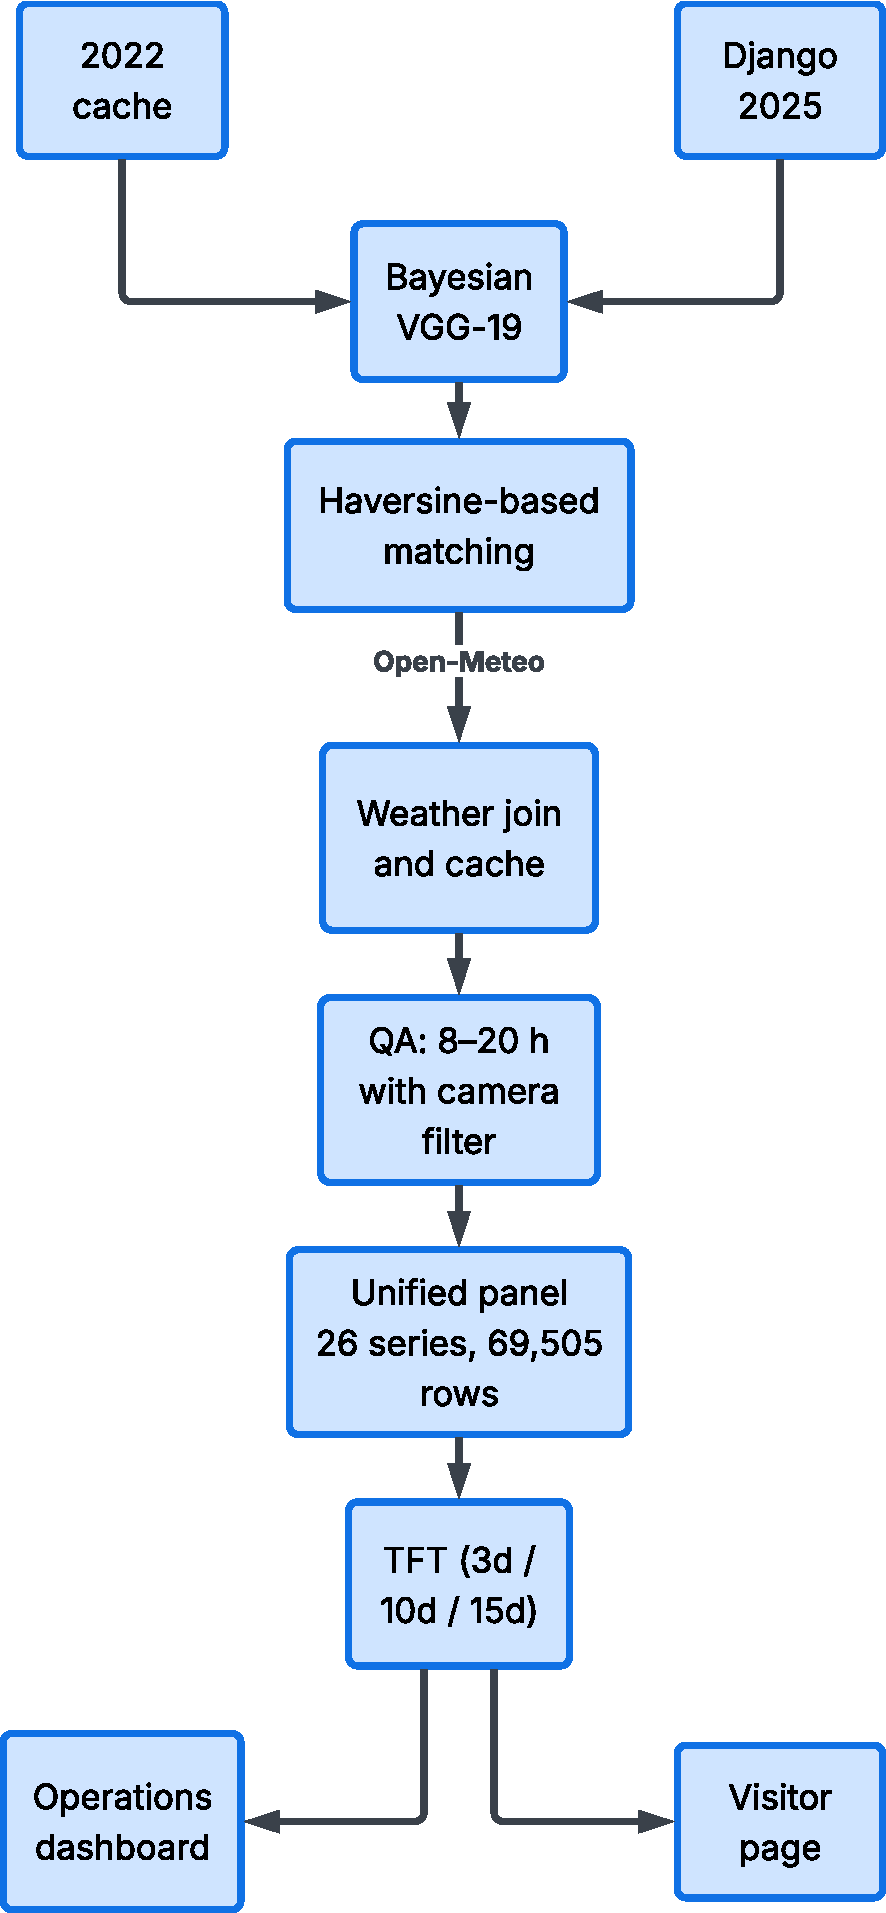
\includegraphics[width=0.92\linewidth]{figures/fig_pipeline_full.pdf}
    \end{center}
    \caption{End-to-end production pipeline: webcam images feed the Bayesian VGG-19 crowd counting model, hourly counts are joined with Open-Meteo weather and filtered to the clean dataset (26 series, 69{,}505 rows), and the TFT serves the dashboard and visitor pages.}
    \label{fig:pipeline_full}
\end{figure}

\subsection{Image-Based Count Estimation}\label{sec:gt}

Per-image crowd counts are produced by the Bayesian VGG-19 crowd counting model of Ma~\emph{et~al.}~\cite{Ma2019Bayesian}, applied to each frame extracted from the webcam streams. Density-map based crowd counting (CSRNet~\cite{Li2018CSRNet} and the family of CNN approaches surveyed in Sindagi and Patel~\cite{Sindagi2018Survey}) forms the broader methodological context. The upstream project~\cite{SanchezGarcia2024TFG} compared this Bayesian model with a point-based one (P2PNet): on the full set of beaches the two were about equally accurate, but the Bayesian model coped better with noisy images, kept improving as more data was added, and was much cheaper to train, so it was the one kept for the pipeline. The crowd counting model is supporting input rather than a contribution: we reuse pretrained weights, run inference frame by frame, and aggregate to hourly resolution by mean. Human annotations were used to fine-tune the crowd counting model but no per-beach human-labelled validation set is computed in this thesis; a per-camera validation logic (seasonality slope, Cohen's $d$ and a peak-vs-shoulder fallback) acts as the de-facto sanity filter, removing cameras where the crowd counting model clearly malfunctions.

\subsection{Weather Source Selection}

Two weather sources were available: Open-Meteo~\cite{OpenMeteo2024}, an aggregator of ECMWF/IFS, NOAA/GFS, ICON and other national-NWP models, and AEMET, the Spanish national weather service. A diagnostic was run on the pre-filter dataset comparing TFT accuracy with and without the AEMET features. Adding the AEMET hybrid changed accuracy inconsistently across runs on the 2022 dataset, from a clear regression to occasional gains, so the accuracy evidence alone was inconclusive. The decisive reason was operational complexity. AEMET's station network is sparse relative to the 22 beach locations, so using it would require building a spatial interpolation model to reach the sites without a nearby station --- an extra pipeline stage that Open-Meteo already provides through its per-beach interpolation. AEMET was therefore dropped, and only Open-Meteo features survived into the final models. Dropping AEMET as a separate source does not discard its information. Open-Meteo has no Spanish national model, but the global models it serves (ECMWF IFS, GFS, ICON) assimilate regional observations shared through the WMO network, so much of the same underlying data is plausibly already present indirectly rather than as a separate AEMET feed.

\subsection{Daytime Filter}

VGG-19 crowd counts are unreliable in low-light conditions. Five strategies for handling night hours were considered: keeping only the daytime hours, keeping all 24 hours, setting the night counts to zero, replacing them with the daytime first quartile, and replacing them with the daytime minimum. The three imputation strategies bias the validation metric: the model learns to reproduce the imputed constant for night hours, and validation contains the same constant, so MAE on those hours is artificially low. The reported overall MAE then mixes a real daytime error with an artificially deflated night error. The fixed 8:00--20:00 filter (thirteen daytime hours per day) avoids the metric bias entirely and was adopted as the project-wide convention. Figure~\ref{fig:solar_hour} supports the choice: the daytime band of crowd counts tracks the solar-radiation curve in summer and collapses in winter, while the grey shaded zone (00:00--07:00 and 21:00--23:00) shows the noisy, near-zero band that the filter excludes.

The 8:00--20:00 boundary was chosen empirically from the activity
distribution: in summer (Jun--Aug), the 07:00--09:00 window contains
approximately 11\% of daytime activity and the 17:00--20:00 window
approximately 6\%, with the bulk concentrated between 09:00 and 17:00.
Excluding both shoulder windows discards roughly 17\% of summer activity but
removes the sunrise and sunset transition where the VGG-19 crowd counting model is least
reliable. A narrower winter-specific window (09:00--17:00) was considered and
rejected on simplicity grounds: a fixed filter is reproducible without
seasonal calendar lookups and decouples the data pipeline from
season-definition assumptions.

\begin{figure*}[!t]
    \begin{center}
        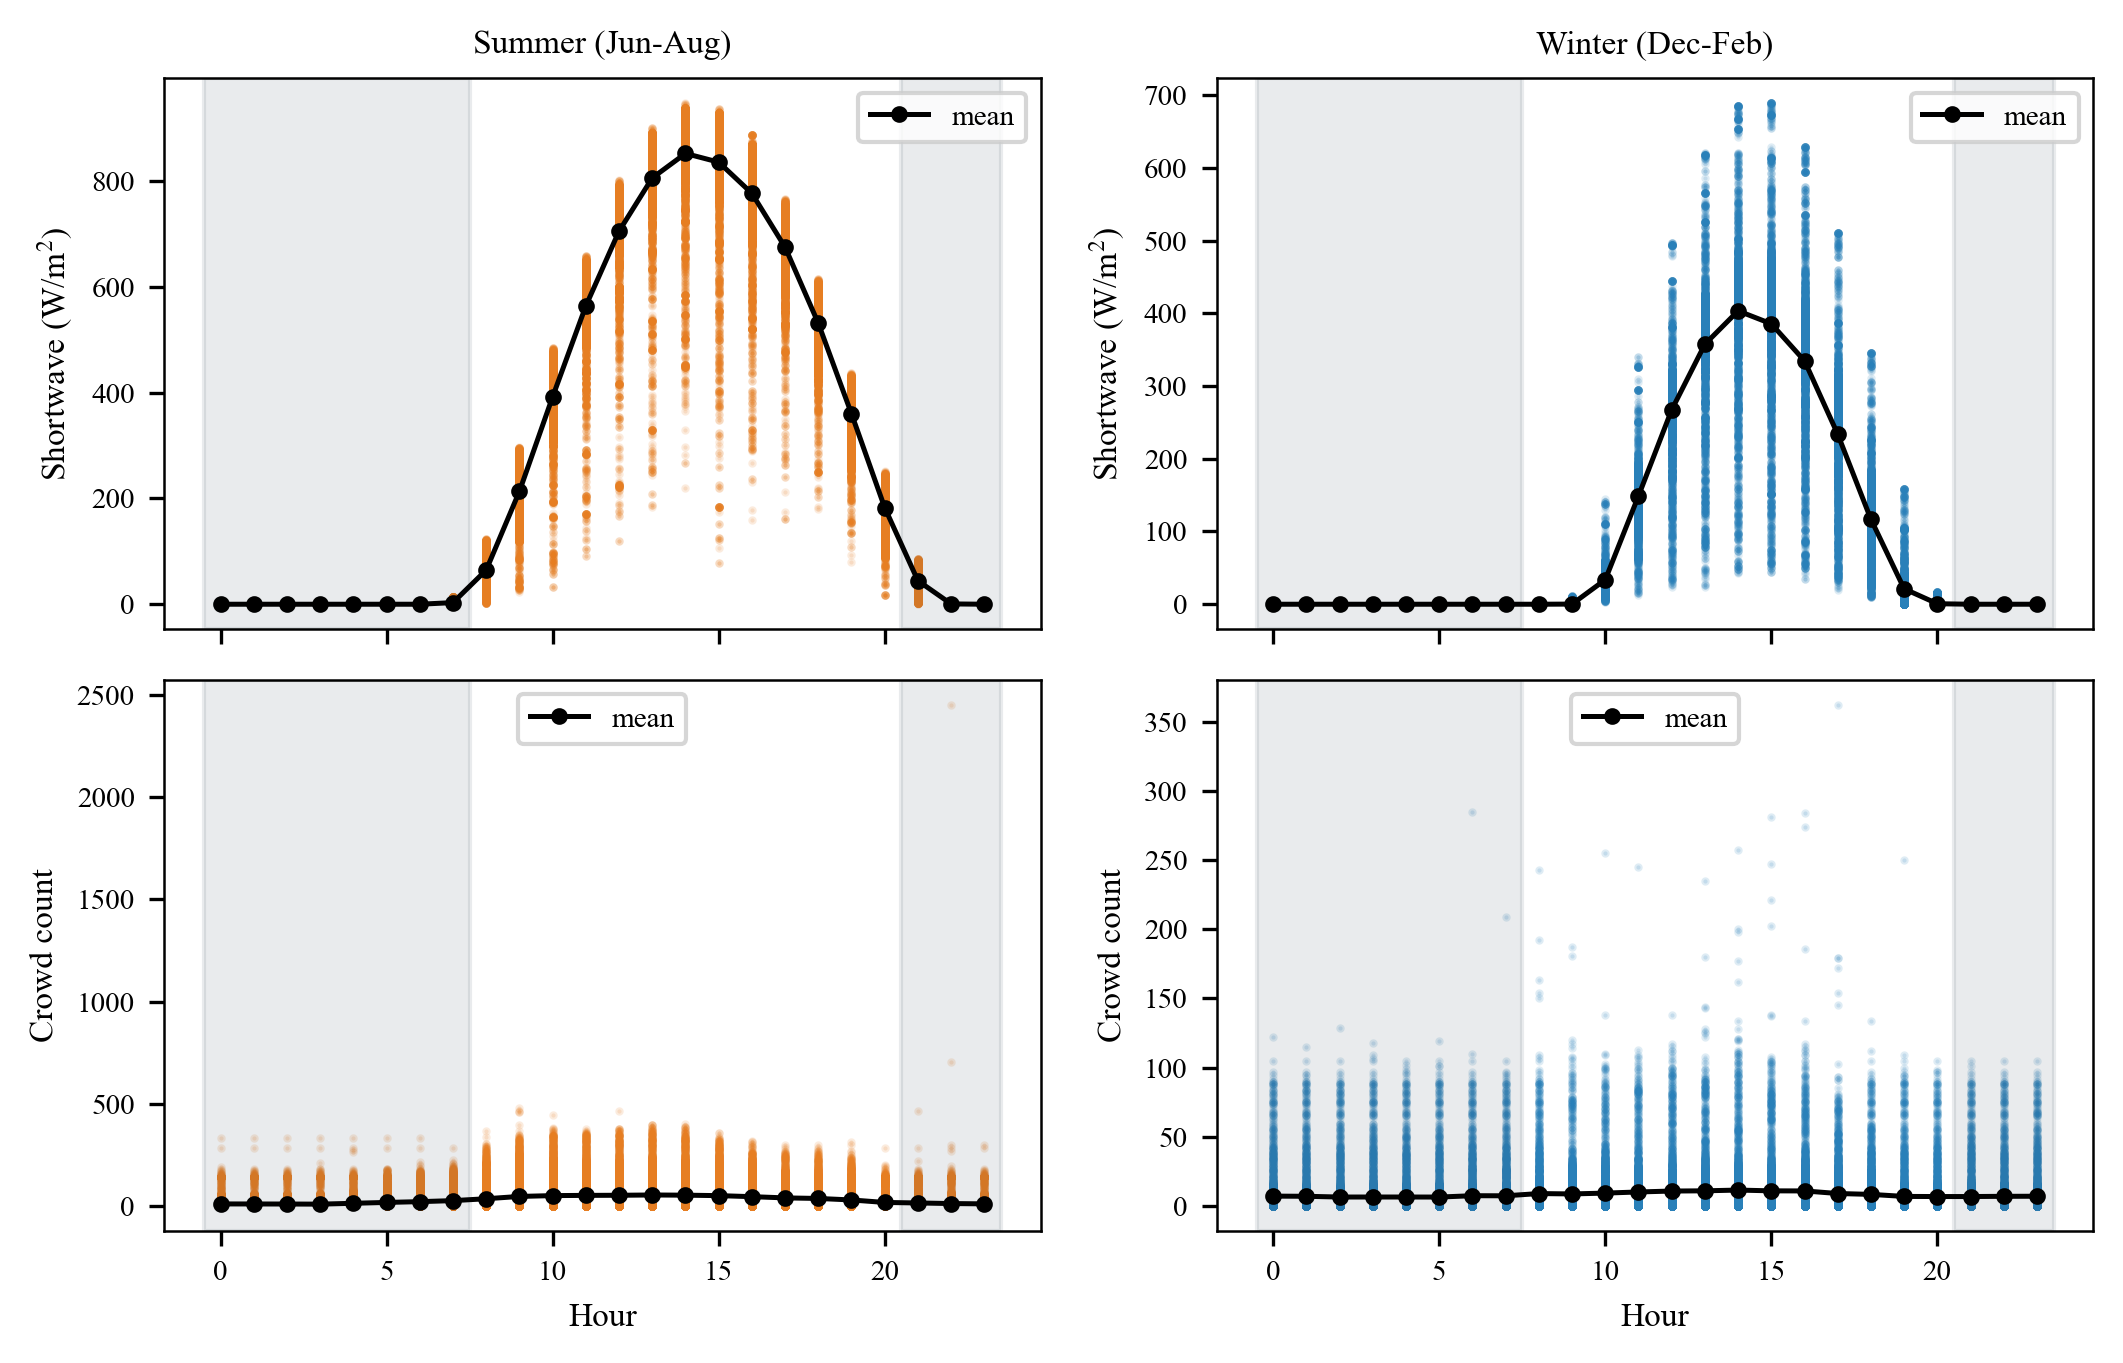
\includegraphics[width=\textwidth]{figures/fig_solar_vs_crowd_by_hour.png}
    \end{center}
    \caption{Solar radiation (top) and crowd count (bottom) by hour, summer (left) vs winter (right). Grey band marks the hours excluded by the 8:00--20:00 daytime filter.}
    \label{fig:solar_hour}
\end{figure*}

\subsection{Camera Validation by Seasonality Slope}\label{sec:camval}

Candidate series are screened for a genuine seasonal signal before entering the training dataset (Figure~\ref{fig:camval}). A prior cleaning pass removes frozen-sensor periods: any window whose rolling coefficient of variation (48 daytime samples, about 3.7 days) falls below 0.05 is dropped, since a near-constant count signals a stuck or frozen camera rather than real occupancy. For each series we compute two complementary measures of seasonality between the summer and winter populations: the summer-to-winter mean ratio and Cohen's $d$. The ratio captures the magnitude of the seasonal swing but is unstable when the winter mean is near zero and ignores the within-season spread; Cohen's $d$ standardises the summer--winter gap by that spread, so it detects a clean separation even when the ratio is modest, and a large but noisy swing does not fool it. Because each measure has a blind spot the other covers, a series is kept when it is clearly seasonal by \emph{either} one --- summer/winter ratio above $2\times$ or Cohen's $d$ above $0.5$ (a medium effect) --- and is otherwise flagged as suspect and excluded. The permissive ``either'' rule avoids dropping a genuine beach that one measure misses; the excluded harbour cameras fail both. Figure~\ref{fig:cohen} plots the per-series Cohen's $d$, the effect-size companion to the ratio. On the Django (2025--2026) dataset the ranking is clear: strong-signal beaches (Cala Vedella, Playa de Palmira, Es Pujols, and others) have summer/winter ratios well above $5\times$ (the strongest exceeds $50\times$) and clearly belong in the training set, while a small group of harbour cameras (the Port d'Andratx group, the Marina and S\'oller-Santa Catalina) sit at or below $1\times$ with Cohen's $d$ near zero, indicating no seasonal beach signal, and are excluded. A camera that fails the test typically frames a harbour, a clifftop or a coastal road rather than a beach, so its counted crowd carries no seasonal structure for the model to learn (Figure~\ref{fig:seasonal_grid}, bottom row). The same procedure is repeated on the 2022 cache dataset, with similar exclusion rates.

\begin{figure*}[!t]
    \begin{center}
        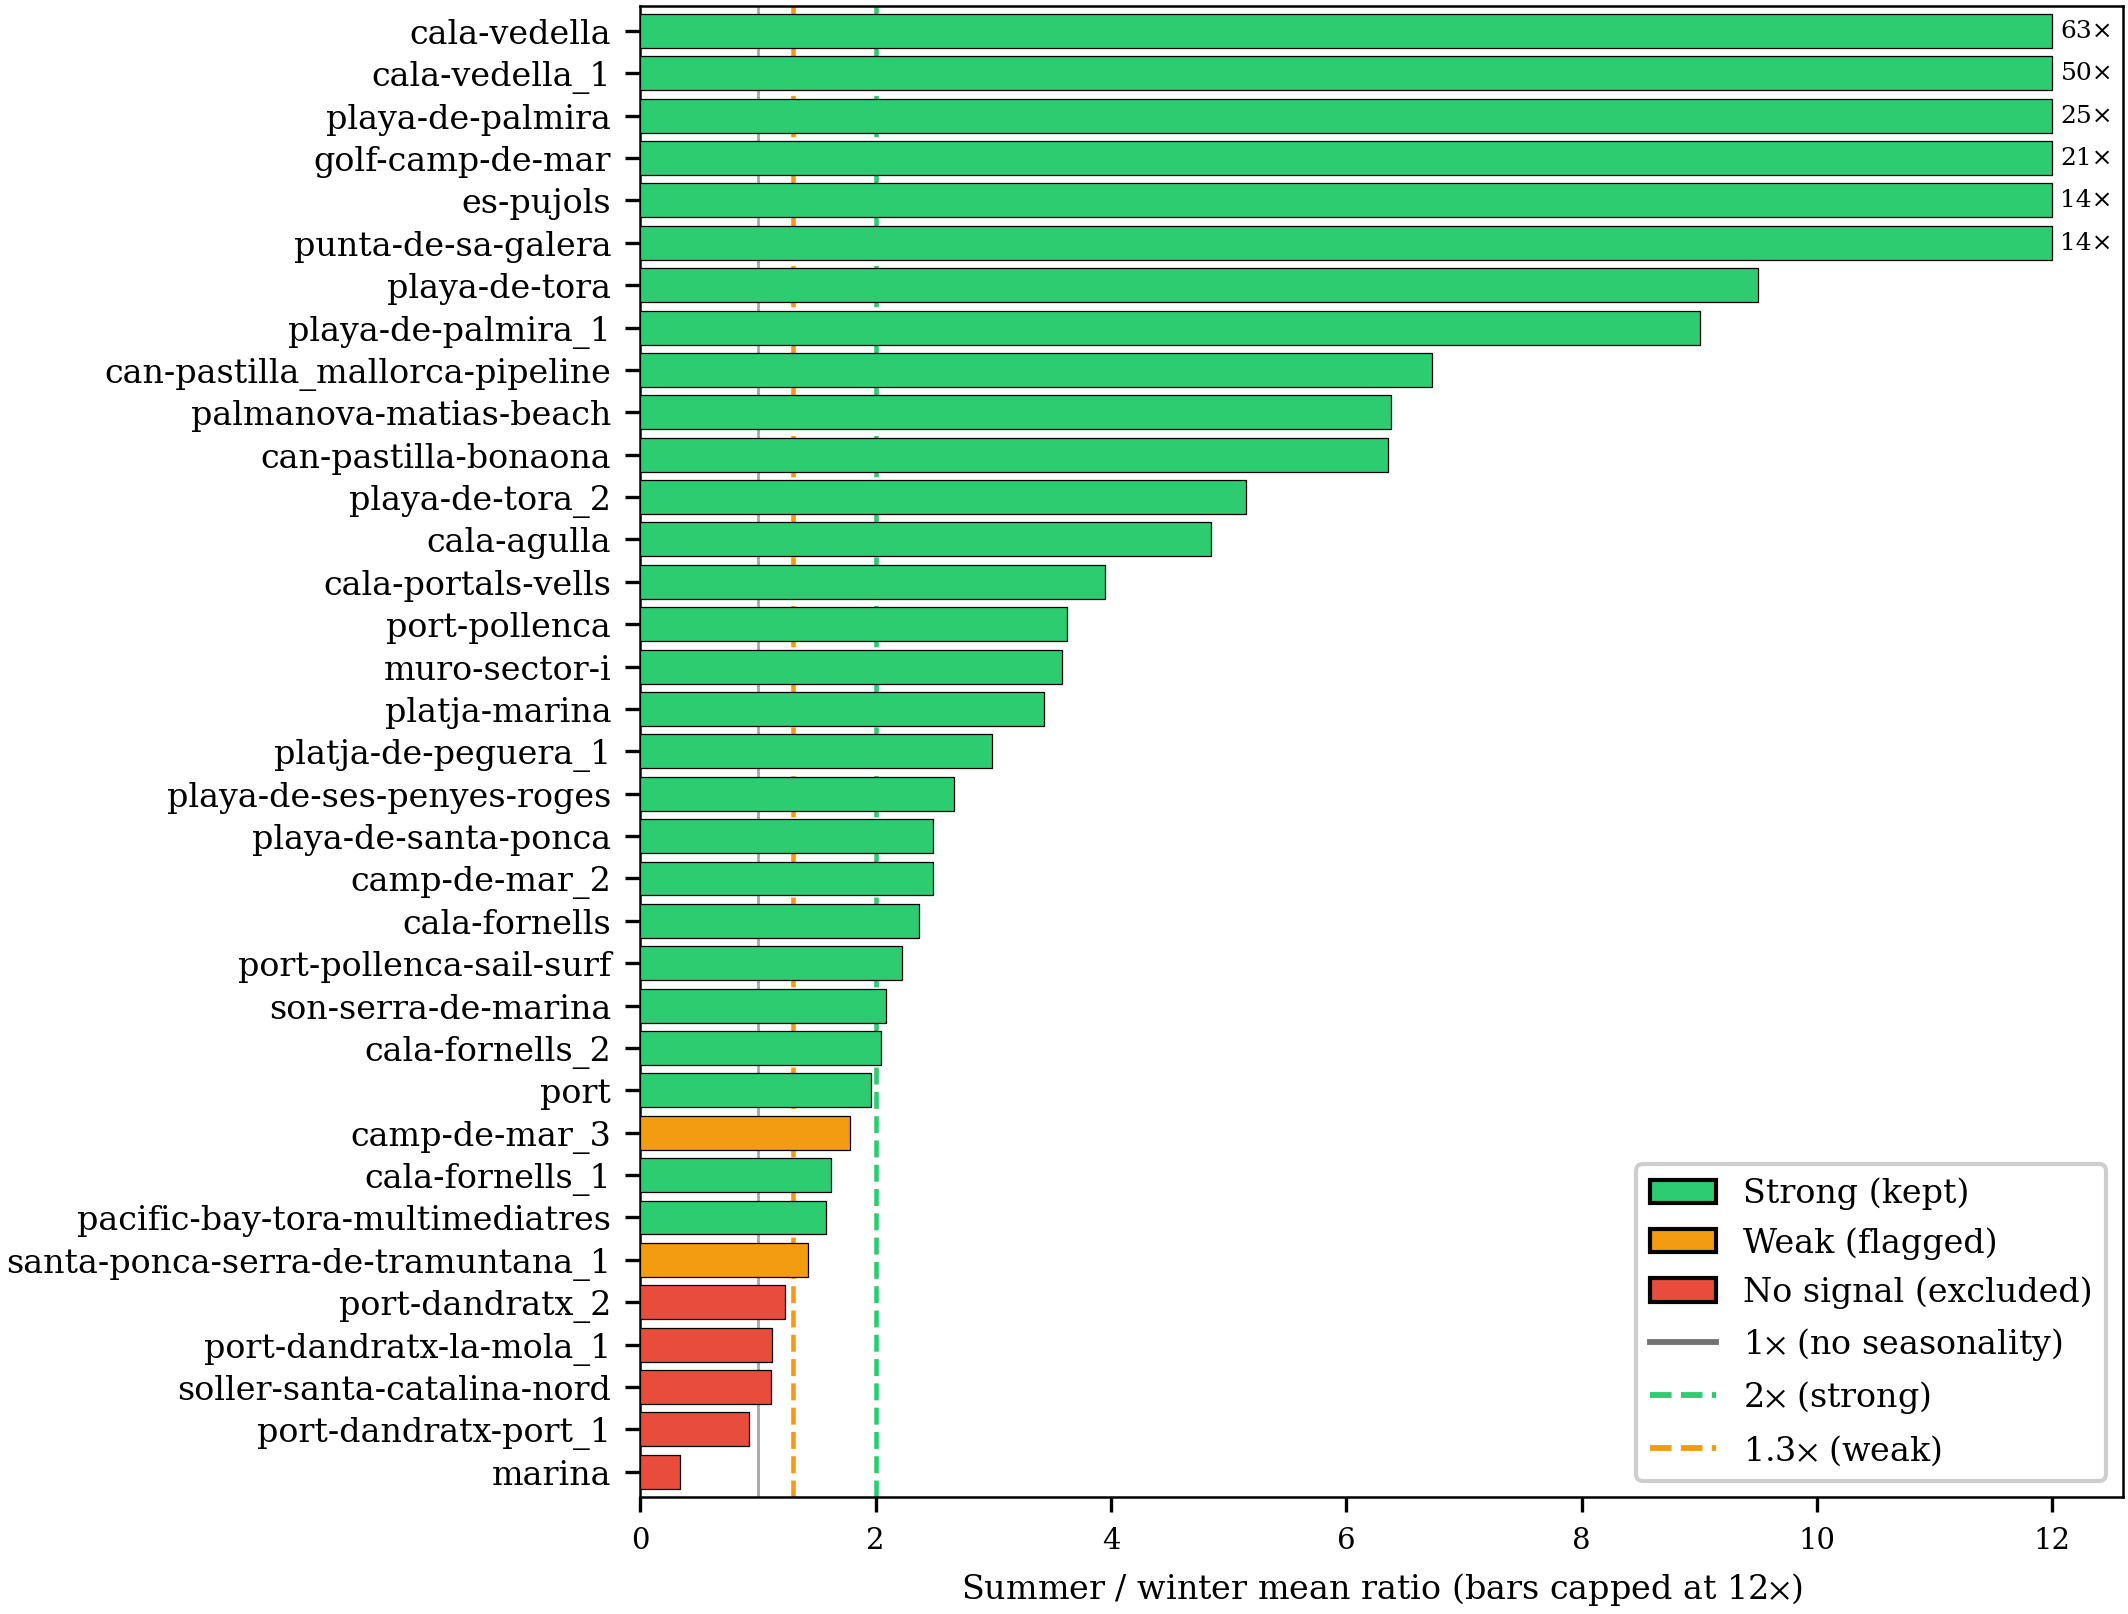
\includegraphics[width=\textwidth]{figures/fig_camval_scatter.png}
    \end{center}
    \caption{Camera validation on the Django (2025--26) dataset: per-series summer/winter mean ratio, sorted and coloured by seasonality class: strong (ratio $>2\times$ or Cohen's $d>0.5$) is kept; weak (ratio $>1.3\times$) and no-signal are both excluded. Bars are capped at $12\times$ for display.}
    \label{fig:camval}
\end{figure*}

\begin{figure*}[!t]
    \begin{center}
        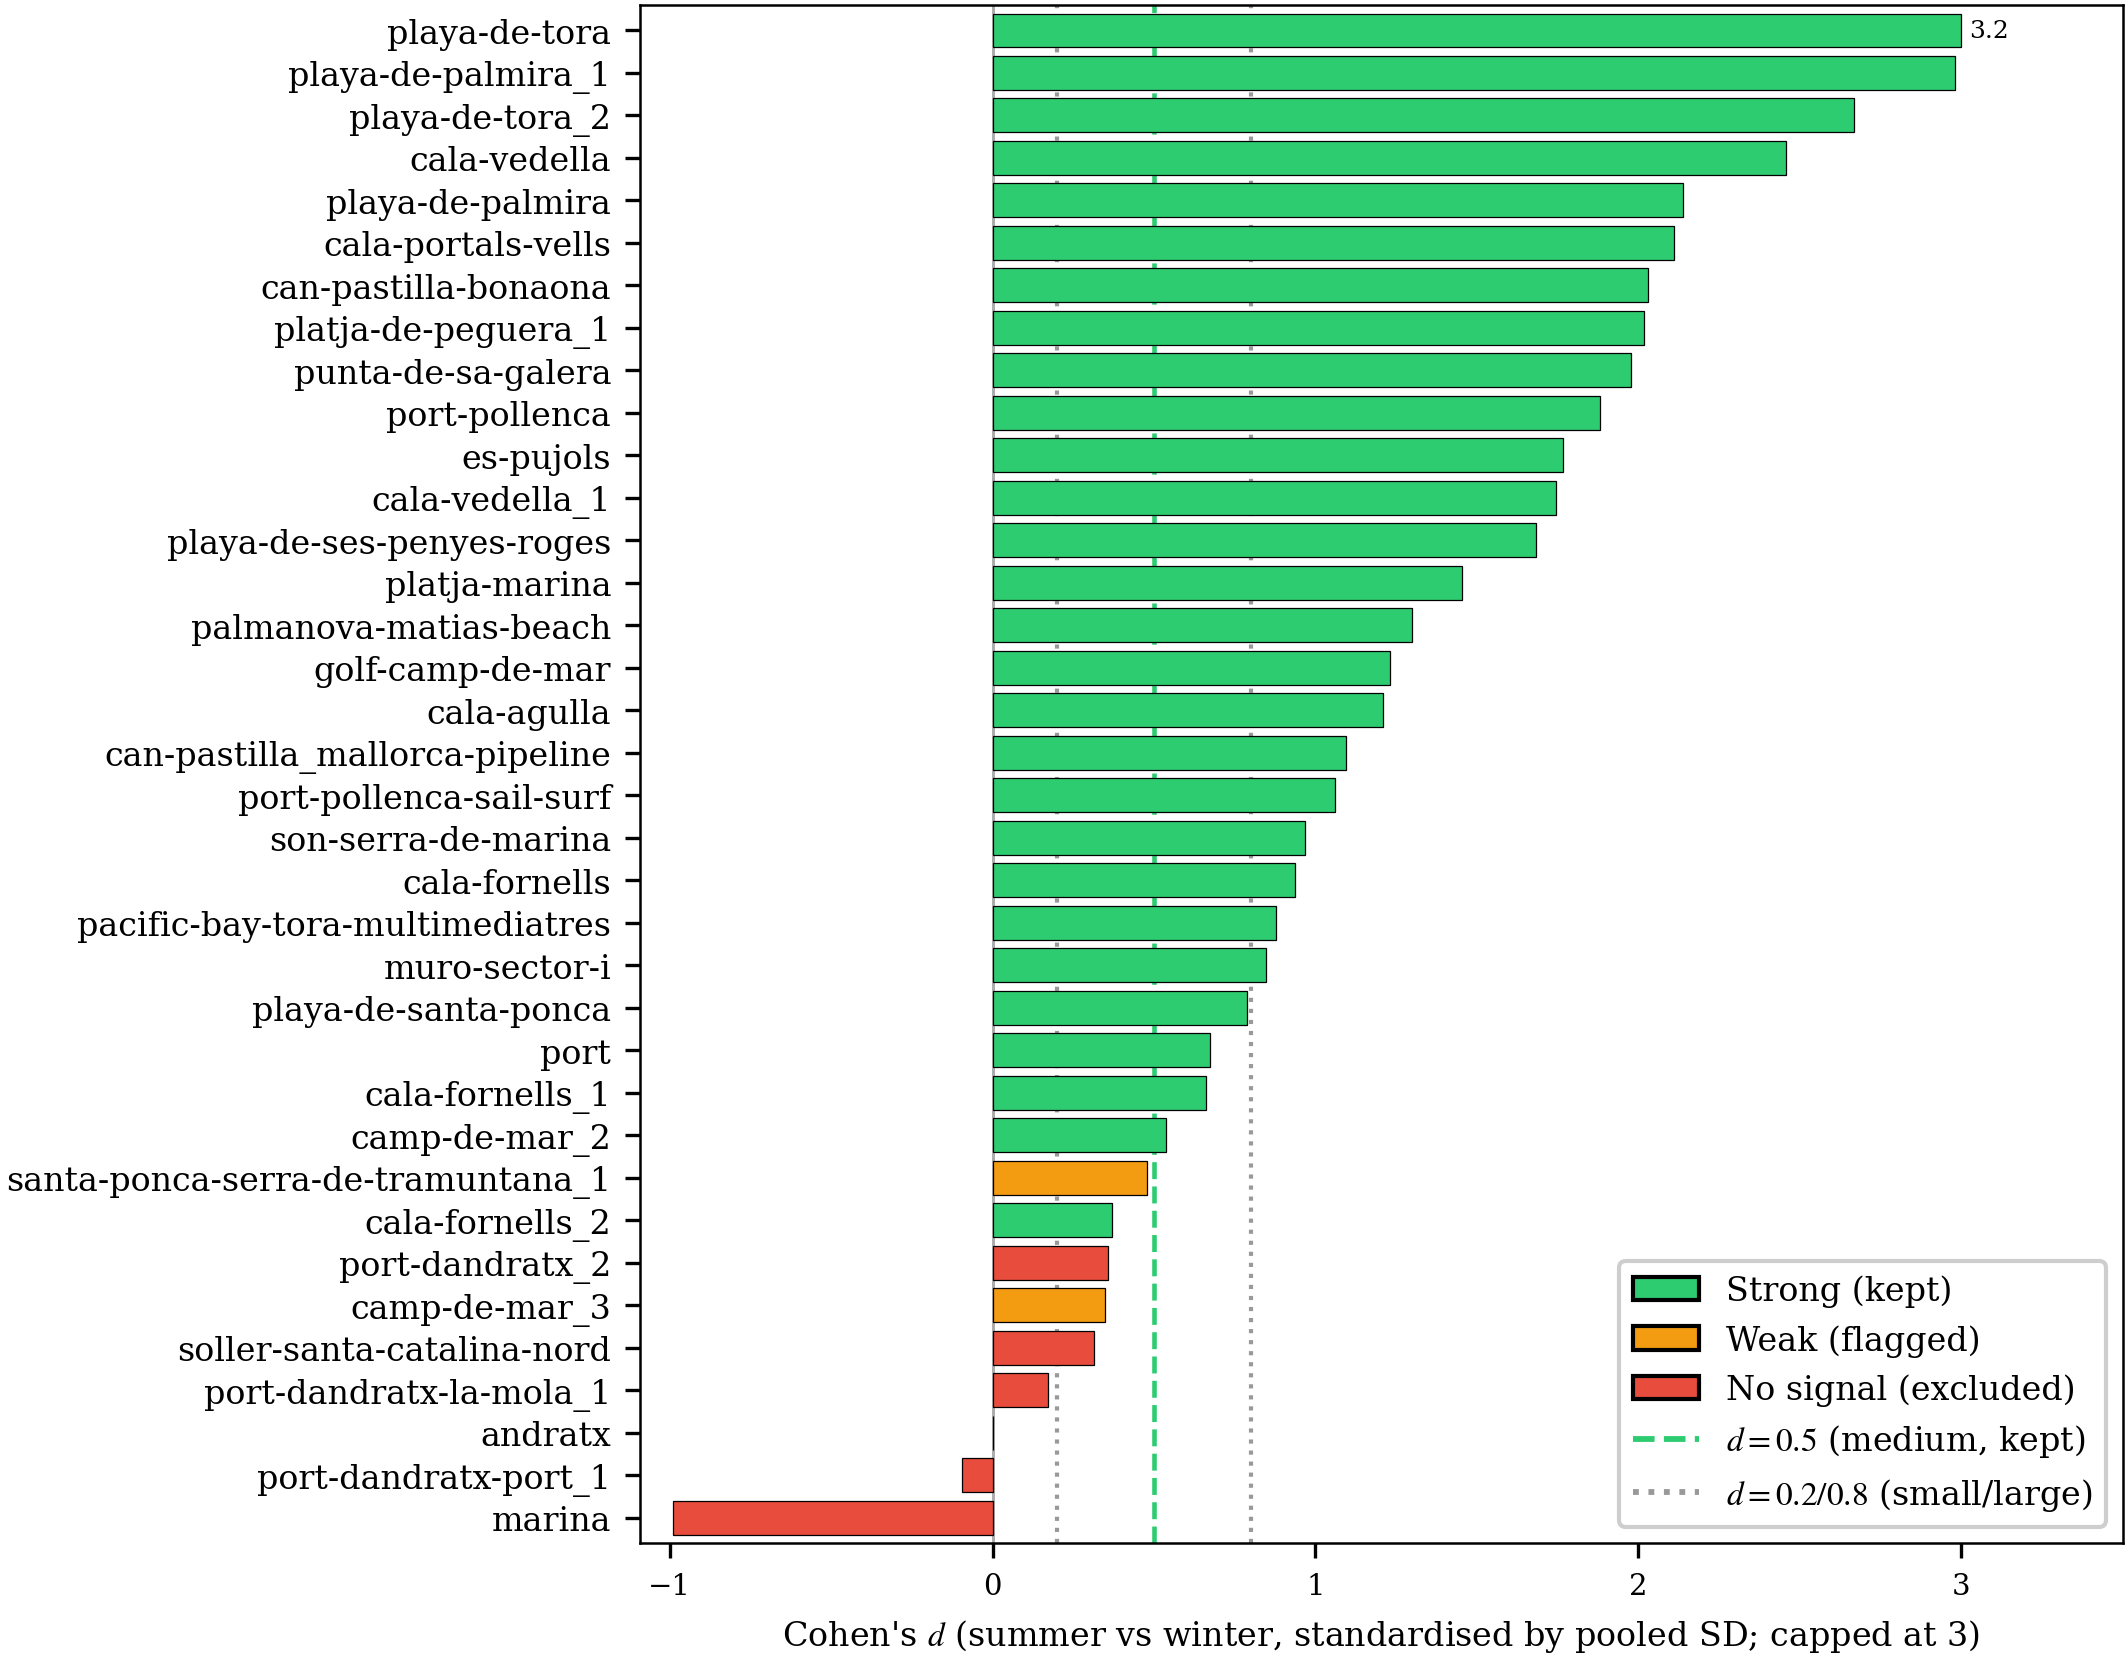
\includegraphics[width=\textwidth]{figures/fig_cohen_scatter.png}
    \end{center}
    \caption{Per-series Cohen's $d$ (the effect-size companion to the summer/winter ratio of Figure~\ref{fig:camval}), sorted and coloured by the same seasonality class. A series is kept when $d>0.5$ or the ratio exceeds $2\times$: the green bars left of the $d=0.5$ line are kept by the ratio, not by $d$ --- the complementarity the two measures provide. Negative $d$ (the harbour cameras) means winter is busier than summer.}
    \label{fig:cohen}
\end{figure*}

Figure~\ref{fig:seasonal_grid} contrasts a kept beach with an excluded camera at the same clock hour across the four seasons. The top row (Sant Antoni de Portmany) fills through spring and summer and empties in winter, the swing the test detects; the bottom row (a coastal-road view) barely changes. The Bayesian VGG-19 crowd counting model is applied to every such frame to produce hourly counts, and the seasonality test cleanly separates the swinging beaches (Cohen's $d$ in the ``large'' range) from the flat cameras.

\begin{figure*}[!t]
    \centering
    \makebox[0.25\textwidth][c]{\footnotesize Winter}\makebox[0.25\textwidth][c]{\footnotesize Spring}\makebox[0.25\textwidth][c]{\footnotesize Summer}\makebox[0.25\textwidth][c]{\footnotesize Autumn}\\[2pt]
    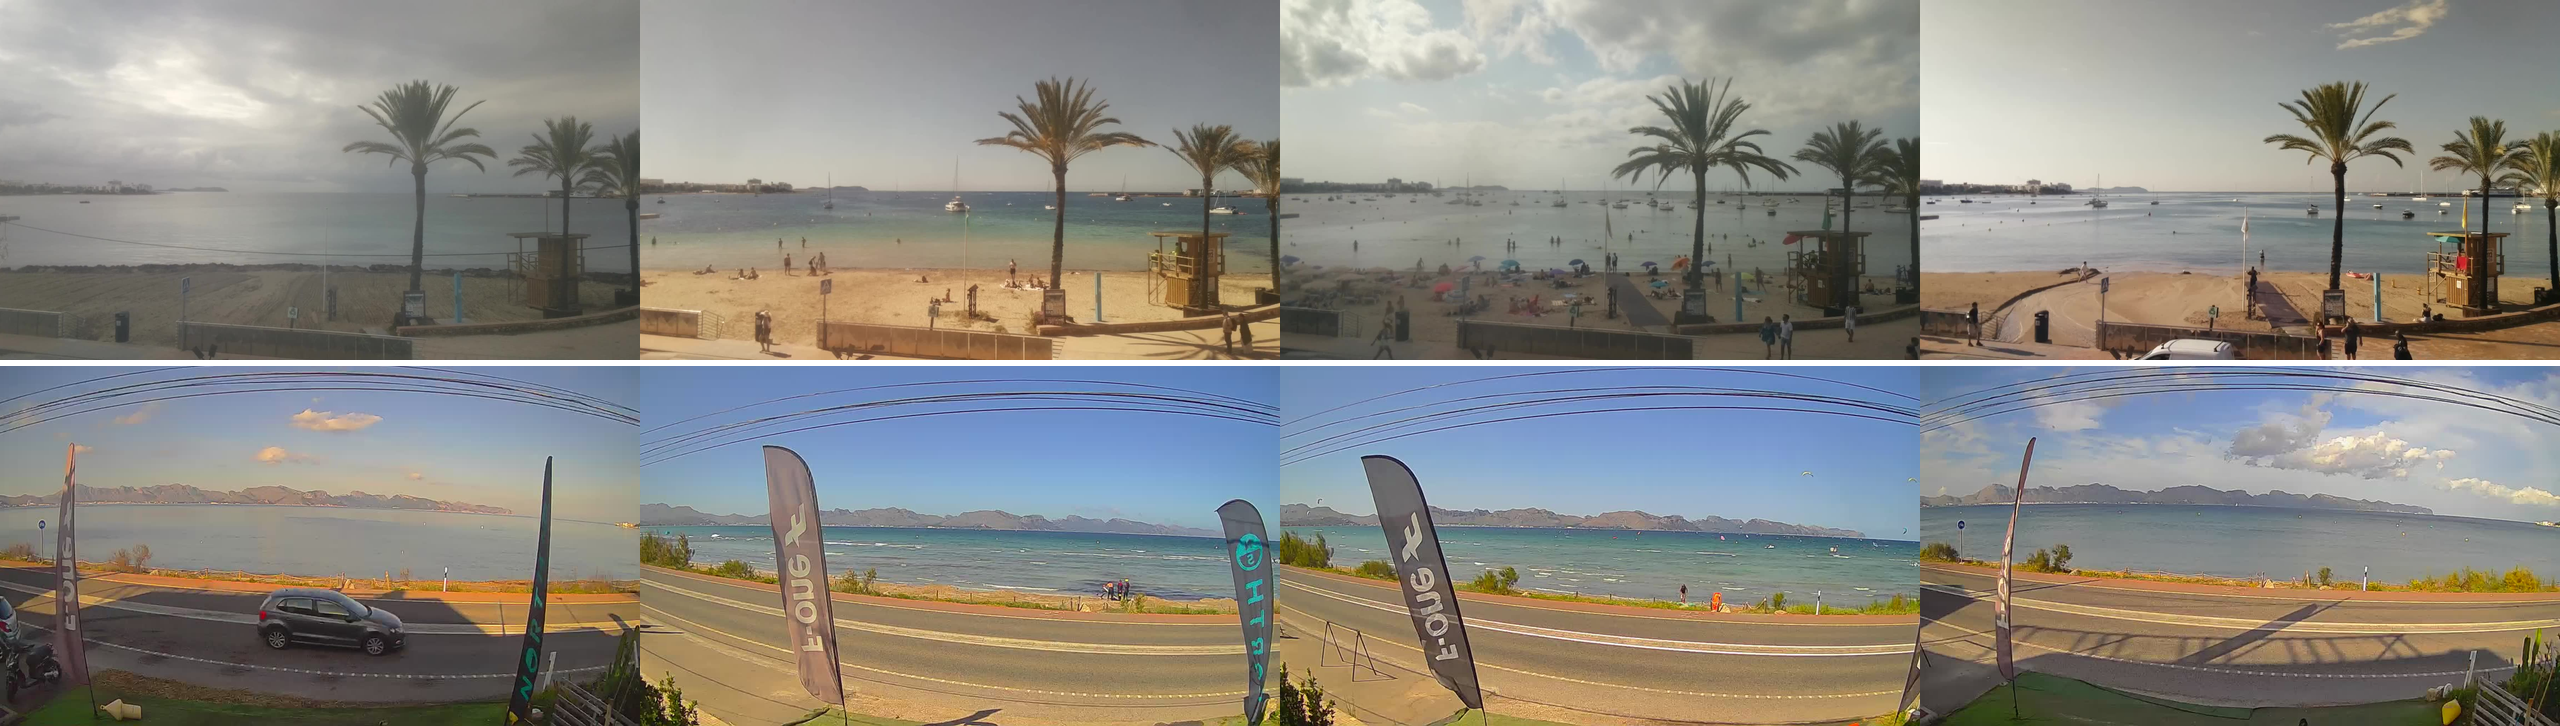
\includegraphics[width=\textwidth]{figures/fig_seasonal_grid.png}
    \caption{Same-time (14:00) webcam snapshots across the four seasons (columns left to right: winter, spring, summer, autumn), sampled at one clock hour so the contrast is seasonal, not diurnal. \emph{Top:} a kept beach (Sant Antoni de Portmany) fills through spring and summer and empties in winter --- the seasonal swing the test is built to detect. \emph{Bottom:} an excluded camera (an Alc\'udia coastal-road view) stays visually flat across all four seasons, carrying no beach-occupancy signal, which is why the seasonality test drops it.}
    \label{fig:seasonal_grid}
\end{figure*}





\subsection{Outlier Capping}\label{sec:cap}

The Bayesian VGG-19 crowd counting model occasionally produces spurious spikes (a glare frame, a transient foreground crowd at the camera, or a counting artifact) that push the real series far above any plausible beach occupancy. A relative error metric is sensitive to exactly these few rows, so, if left unchecked, they distort both training and evaluation. We therefore cap the \emph{real} crowd count per series: within each beach series, daytime positive counts above $k\cdot\mathrm{P90}$ (with $k=1.5$ and $\mathrm{P90}$ the series' 90th percentile of real daytime counts) are clamped down to that threshold. The cap is selective rather than a winsorisation at the P90 itself: only the tail above $1.5\times$ the P90 is touched, roughly 1--2\% of daytime-positive rows, so genuine peak-demand days survive intact.

Three properties keep the cap from contaminating the comparison. First, it is applied to the \emph{actual} counts only, never to model predictions, so each model is still scored against a cleaned but real target. Second, it is applied consistently to both the training targets and the evaluation actual values; capping one and not the other would bias the comparison. Third, the P90 capacity denominator of the relMAE metric (see Section~\ref{sec:metric}) is invariant under the cap: because only counts strictly above $1.5\times$P90 are clamped down to $1.5\times$P90, a value that still sits above the 90th percentile, the P90 quantile itself is unchanged, so the cap cannot shrink the normaliser and flatter the reported error. Raw counts are stored on disk and the cap is applied at load time by a single shared routine, so every training, validation and scoring path sees the identical cleaned series.

\section{Methodology}\label{sec:method}

This section covers the experimental setting, the evaluation metric, the validation design and the model-selection methodology.

\subsection{Experimental Setting}\label{sec:setup}

All models are trained and evaluated on a single NVIDIA RTX~A6000 GPU (48~GB VRAM), the deployment hardware; its memory ceiling sets the maximum trainable horizon probed in Section~\ref{sec:horizon_ceiling}. The offline evaluation runs under Python~3.13.5 with neuralforecast~3.1.4, PyTorch~2.9.1, Optuna~4.7.0, XGBoost~3.1.3, pandas~2.3.3, NumPy~1.26.4, scikit-learn~1.7.2 and SciPy~1.16.3; the servable models were trained on the same GPU under Python~3.10 with the same neuralforecast~3.1.4. Every random source is seeded with $\text{SEED}=42$ --- the Optuna Tree-structured Parzen Estimator (TPE) sampler, the NeuralForecast/PyTorch model initialisation and the XGBoost \texttt{random\_state} --- so the runs are reproducible.

\subsection{Evaluation Metric}\label{sec:metric}

Two metrics are reported throughout: \emph{overall} relative MAE (computed over all rows in the test partition, all twelve months) and \emph{season} relative MAE (computed over rows with month in April through September). Relative MAE for a series $s$ is the mean absolute error of that series normalised by a per-series capacity $C_s$,
\[
  \mathrm{relMAE}_s \;=\; \frac{1}{N_s}\sum_{t=1}^{N_s}\frac{|\hat{y}_{s,t}-y_{s,t}|}{C_s},
\]
and the reported figure is the mean of $\mathrm{relMAE}_s$ across series. Normalising per series, rather than pooling all residuals against one global scale, makes the metric comparable across beaches of very different size. The coefficient of determination ($R^2$) is reported as a secondary goodness-of-fit measure; $R^2_\text{med}$ denotes its per-beach median.

The capacity $C_s$ is the per-series P90 of the \emph{actual} daytime counts: it measures error relative to how busy each beach typically gets, and it is computed on the training rows only, so the test window never enters the normaliser. Every table in this thesis uses this same capacity, and the deployed system classifies occupancy against it too, so all numbers are read on one scale. Every count in the dataset is itself a VGG-19 estimate, so each relMAE measures agreement with that estimator and is an upper bound on accuracy against true human occupancy rather than a comparison to it.

Where two competing models are compared on the same paired test set, the primary statistical test is the Diebold-Mariano test~\cite{DieboldMariano1995} with HAC variance and Harvey--Leybourne--Newbold small-sample correction~\cite{Harvey1997DM}; the Wilcoxon paired signed-rank test~\cite{Wilcoxon1945} is reported alongside as a robustness check. DM is chosen as the primary test deliberately: it weights the loss differential by magnitude rather than by rank, which is the operationally correct behaviour for this problem because the highest-magnitude errors occur on peak-demand days (Saturdays in summer) whose forecast accuracy carries disproportionate weight for public-sector operational decisions. A model whose largest residuals concentrate on those peak days should be penalised more heavily than a model whose residuals are spread uniformly; DM does exactly that, while a rank-based test would dilute the peak-day signal. Wilcoxon is retained as a sanity check that the DM ranking is driven by a systematic gap, not by a small number of outlier observations.

Overall relMAE under-states the in-season error. Winter occupancy in the Balearics is low and tightly clustered: across the dataset the winter (Dec--Feb) hourly count distribution has median 13 users and inter-quartile range 6--22, with a dataset-wide P90 of 30, against summer (Jun--Aug) median 52 and dataset-wide P90 of 176. Most beaches sit in the 10--20 user range during winter, with a handful of harbour/promenade cameras (e.g., \emph{Alcúdia Sa Marina} at $\sim 170$ users) carrying year-round traffic. A trivial predictor that outputs the per-series mean already achieves overall relative MAE in the 0.10--0.13 range simply by being approximately correct on the low-variance winter half of the year. Most of the apparent overall-MAE improvement that any real model produces is therefore a winter-window artifact and does not reflect any discriminative power the model has acquired.

Season relMAE measures what stakeholders actually care about. Both stakeholder groups identified in the introduction (public-sector consumers of the FUEIB API and visitors planning trips) engage with the model during the high season. Public-sector operational demand peaks in summer, and visitor trip-planning queries are summer-bound. The season metric isolates the setting where occupancy varies substantially with weather and calendar.

Whenever a single number is cited as the primary figure for a model or experiment, it is the season relative MAE. Overall relMAE is reported as a secondary figure for completeness and for comparison with non-Balearic studies.

\subsection{Experimental Design: Four Validation Protocols}\label{sec:design}

All three families (TFT, LSTM and XGBoost) are validated under four complementary protocols, so that no single train/test split drives the conclusion. The two described in this section --- cross-year transfer and walk-forward cross-validation --- run on the capped data over the 8:00--20:00 daytime window and take the per-series P90 season relMAE as the primary metric; the other two are the operational field evaluation on live data (Validation~3, Section~\ref{sec:prod}) and the multi-scenario check across independent windows (Validation~4, Section~\ref{sec:a2}).

Validation~1 (cross-year transfer, also called domain transfer) trains the models on the 2022 cache era and validates them on the entirely separate 2025--2026 Django dataset. The purpose of this split is to check that a model has learned the generalisable drivers of beach occupancy, the weather, calendar and per-beach patterns, rather than memorising the 2022 period, so that what it learns applies to data it never saw. Because a multi-year gap separates the two eras, the split is a strict test of that ability: how well a model trained on one period transfers to later years, and, for beaches present only in the later era, to sites it never saw in training.

Validation~2 (in-distribution walk-forward cross-validation) splits the full dataset into $N$ expanding folds (four in the reported run); each fold trains strictly on all data before its cut-off (expanding window) and validates the next contiguous window, so there is no look-ahead. The per-fold predictions are pooled and scored exactly as in Validation~1. This protocol measures accuracy when recent in-distribution history is available, which is the operating condition of the deployed system: a scheduled job periodically retrains on the most recent months.

To keep Validations~1 and~2 on identical logic, both are produced by a single evaluation routine that, for each horizon, restricts every family to the \emph{identical} set of matched (beach, timestamp) rows before scoring, computes the per-series P90 relMAE on those rows, and runs the Diebold-Mariano test between families on the same rows. Because the row set, the normaliser and the significance test are held fixed across protocols, the ranking reflects the models rather than differences in coverage. Validation~3, the operational field evaluation (see Section~\ref{sec:prod}), re-scores the deployed models on the same per-series P90 capacity; Validation~4, the multi-scenario check (see Section~\ref{sec:a2}), extends the cross-family comparison to three independent windows on that same capacity.

\subsection{Horizon-set Selection}

The forecast is served at three horizons relevant to municipal operations: short term (about 3 days), tactical (about 10 days) and strategic (about 15 days).

The initial target set was 3, 14 and 30 days. An empirical horizon-ceiling probe on the deployment GPU (see Section~\ref{sec:setup}) trained the TFT under FIXED-HP (a fixed hyperparameter set: hidden size 64, 4 heads, dropout 0.05, learning rate $10^{-3}$; see Section~\ref{sec:p3}), with the input window scaled to each horizon, across a coarse-to-fine sweep of $H \in \{168, 360, 444, 528, 720, 1080, 1440, 2160\}$ output steps; the model fits comfortably up to \mbox{$H{=}444$} steps and runs out of memory from $H{=}528$ onwards (see Section~\ref{sec:horizon_ceiling}). Because the memory limit is set by the number of output steps, a 30-day forecast ($H{=}390$ on the thirteen-hour frame) is well within hardware capacity, and the original training-pipeline failure on it was a configuration artifact, not a model-capacity limit. The decisive constraint is external: Open-Meteo's standard Forecast API exposes at most 16 days of forecast for the future-known weather inputs~\cite{OpenMeteo2024}; without forecast values past day 16, no future-known features are available beyond that horizon and the forecast collapses to autoregressive extrapolation that has no purchase on weather-driven variability (consistent with the roughly 10--14 day deterministic-predictability ceiling of Section~\ref{sec:relwork_weather}).

The horizon set was therefore changed to 3, 10 and 15 days. With thirteen daytime hours per day, the resulting forecast horizons are $H \in \{39, 130, 195\}$ output steps (the length the model predicts, distinct from the input window swept in Section~\ref{sec:phase2}). Each horizon serves a specific operational purpose anchored on a verifiable property of the underlying weather inputs:

\begin{itemize}\itemsep0pt
    \item 3 days ($H{=}39$). This is the high-precision tier of the Open-Meteo forecast. The first 2--3 days of every Open-Meteo response are computed by local high-resolution models (1--2~km) and delivered at the native 1-hourly time step. For ECMWF IFS specifically, the 1-hourly native resolution is guaranteed for the first 90 hours; only after that does the API fall back to 3-hourly (90--144~h) and 6-hourly (144--360~h) outputs, interpolated back to 1-hourly in the response. The 3-day forecast in this setting sits entirely inside the 1-hourly native band, which is the range where the future-known weather inputs are most reliable.
    \item 10 days ($H{=}130$). This is the ``this weekend'' horizon, guaranteed to contain the coming weekend: a Monday-morning forecast covers the upcoming Saturday and Sunday, the two peak-demand days of any given week, with margin to spare for late-week scheduling decisions.
    \item 15 days ($H{=}195$). This is the ``next weekend'' horizon, guaranteed to reach the following weekend: a Monday-morning forecast extends through the Saturday and Sunday of the following week, supporting fortnightly planning windows. The choice of 15 days (rather than 14) was made for simplicity: with $H{=}182$ (14 days) a Friday-morning forecast ends Thursday evening of the second week, missing the second Friday entirely; with $H{=}195$ the forecast horizon always reaches the same weekday two weeks out (a horizon guaranteed to contain the coming weekend) for any issuing weekday.
\end{itemize}

\subsection{TFT Architecture and Feature Design}\label{sec:tftfeat}

Figure~\ref{fig:tft_arch} summarises the architecture as instantiated in this work (after Lim~\emph{et~al.}~\cite{LimTFT2021}).

\begin{figure*}[!t]
    \begin{center}
        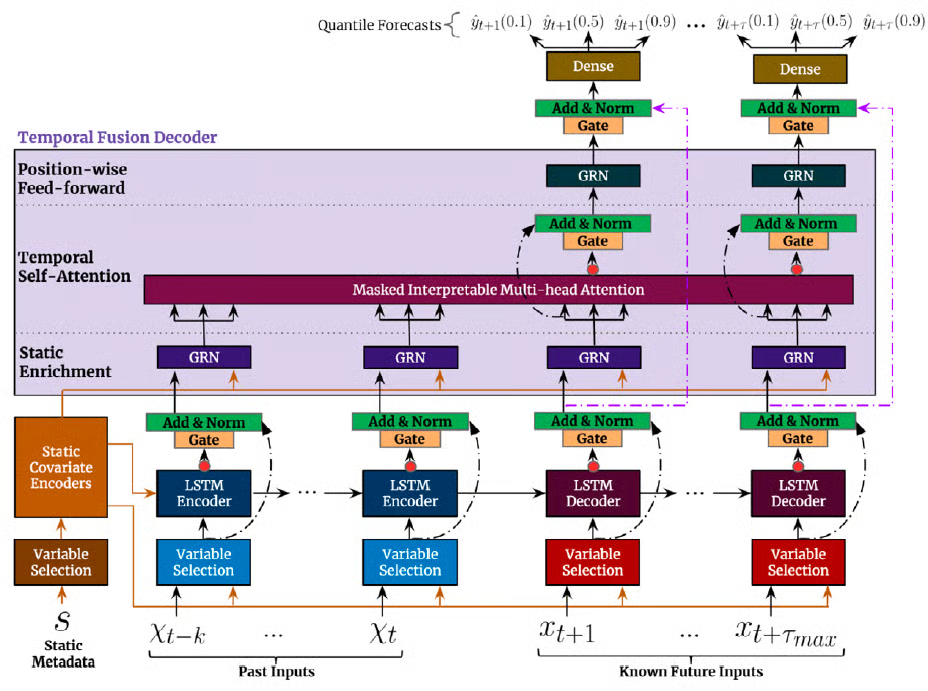
\includegraphics[width=\textwidth]{figures/fig_tft_architecture.png}
    \end{center}
    \caption{Temporal Fusion Transformer data flow as instantiated here: the three-input typology (static, known-future, historical observed), per-stream Variable Selection Networks, static context encoder, LSTM encoder--decoder, interpretable multi-head attention, and quantile output head. Adapted from Lim~\emph{et~al.}~\cite{LimTFT2021}.}
    \label{fig:tft_arch}
\end{figure*}

The Temporal Fusion Transformer~\cite{LimTFT2021} is an attention-based encoder--decoder architecture designed for multi-horizon forecasting on panel data with heterogeneous inputs. It distinguishes three input types at the model interface: \emph{static} covariates (per-series attributes that do not change over time), \emph{known-future} covariates (inputs whose values at every forecast step are known a priori, such as calendar variables and forecast weather), and \emph{historical observed} covariates (inputs available only up to the issuance time, such as past target values and lag-based features). Inputs of every type pass through a \emph{Variable Selection Network}, a gated transformation that learns soft input-importance weights and discards irrelevant variables on a per-step basis, providing native interpretability. A static-context encoder injects per-series identity (e.g., per-beach mean and coefficient of variation in our case) into every block of the temporal pipeline through gated residual networks, so that beach-specific scale and seasonality conditioning is shared across all hidden representations rather than relearned at each step. The temporal pipeline then combines a sequence-to-sequence LSTM encoder over the historical window with an \emph{interpretable multi-head self-attention} block over the forecast window, allowing the decoder to attend across long ranges (here up to 195 steps) while preserving the inductive bias of recurrent processing on the recent past. The output is a quantile-regression head: each forecast step emits a distribution rather than a point estimate, with pinball-loss (quantile-loss) training that yields built-in predictive intervals without a separate calibration stage.

The architecture fits the operational constraints of this pipeline in several ways. Its three-input typology matches the data directly --- static per-beach attributes, calendar and forecast-weather inputs known one step ahead, and historical observations of the target and past weather --- so no reshaping of the features is needed to fit the model interface. The Variable Selection Networks double as a transparency layer for the operator dashboard: the gating weights that drive training also show which inputs the model used at each step, which feeds the per-hour feature tooltip in the hindcast comparison (see Section~\ref{sec:prod}). Multi-horizon prediction is native --- the trained model emits the whole horizon at once, avoiding the error accumulation of autoregressive single-step models at the 15-day target. Together these motivated choosing the TFT over the modern transformer family of Section~\ref{sec:relwork_tsforecast}, none of which combines the three-input typology, the per-step interpretability and the production-ready quantile output in one model (Table~\ref{tab:model-selection}).

Within this architectural skeleton, each variable's input type (static, known-future or observed-only) is fixed by its nature; the design choice is which variables to include, while keeping each type small enough to fit GPU memory at the longest horizon ($H{=}195$).

The features assigned to each of the three input types are listed in Table~\ref{tab:features}.

\begin{table}[!ht]
    \caption{TFT input feature schema: STATIC, FUTURE and OBSERVED-ONLY inputs. Scraped beach attributes were tested as additional STATIC inputs in Phase~1 and rejected.}
    \label{tab:features}
    \begin{center}
    \begin{tabular}{ll}
        \toprule
        Group & Features \\
        \midrule
        STATIC  & per-series mean, per-series CV \\
        FUTURE  & hour, day-of-week, month, \\
              & is\_weekend, is\_summer, \\
              & 2m temperature, apparent temp., \\
              & total cloud cover \\
        OBSERVED-ONLY  & 2--3 weather variables \\
              & (finalised in Phase 1) \\
        \bottomrule
    \end{tabular}
    \end{center}
\end{table}

The five calendar FUTURE features encode the dominant tourism cycles. The three FUTURE weather features are selected on three converging grounds: atmospheric-predictability theory~\cite{Lorenz1963,ECMWF2024}, which places temperature among the most reliably forecastable surface variables at multi-day horizons; the tourism-climate-index literature, where Mieczkowski's TCI weights daytime thermal comfort four times more than other terms~\cite{Mieczkowski1985} and the beach-specific Holiday Climate Index (HCI:Beach) explicitly substitutes cloud cover for sunshine~\cite{ScottHCIBeach2016}; and direct precedent in Castelle~\emph{et al.}~\cite{Castelle2025}, who omit humidity entirely and report temperature as the dominant predictor.

The FUTURE weather triplet was chosen a priori on these converging grounds and fixed in the schema, rather than by an in-sample search, because the known-future inputs must stay reliable at multi-day forecast horizons rather than fit the training window. Humidity-family variables are excluded because they decorrelate fastest at multi-day forecast horizons~\cite{ECMWF2024} and because the comparable Castelle~\emph{et al.}\ study explicitly omits them.

\subsection{Variable Selection Network Importances}\label{sec:vsn}

The Variable Selection Network exposes, as a model output, the soft gating weight (a value in $[0,1]$ that scales each input's contribution) assigned to each input on every stream (the per-input-type feature group: static, known-future or past-observed). Because the project is a publicly-funded deployment whose stakeholders inspect forecast attributions (see Section~\ref{sec:relwork_tsforecast}), these weights are reported here as a published, model-native record of which inputs the model relied on, rather than a post-hoc attribution. Figure~\ref{fig:vsn} shows the per-stream weights for the three deployed models; within each stream the weights are a softmax and therefore sum to one.

The same patterns hold across all horizons. In the \emph{known-future} stream the hour of day dominates (0.55--0.65), with 2m temperature the leading weather input (0.09--0.12): the diurnal cycle is the strongest driver of the forecast, consistent with the temperature-and-hour dominance reported by Castelle~\emph{et~al.}~\cite{Castelle2025}. The \emph{past-observed} stream spreads its weight across the autoregressive observed target (approximately 0.20--0.22), the recent hour signal and shortwave radiation (0.13--0.22), confirming that the model leans on its autoregressive memory --- the mechanism identified in Section~\ref{sec:c2} as the reason the TFT transfers across years where XGBoost fails. The static stream is dominated by the per-series mean (0.85) over the coefficient of variation (0.15): per-beach scale is the static signal the model conditions on.

\begin{figure*}[!t]
    \begin{center}
        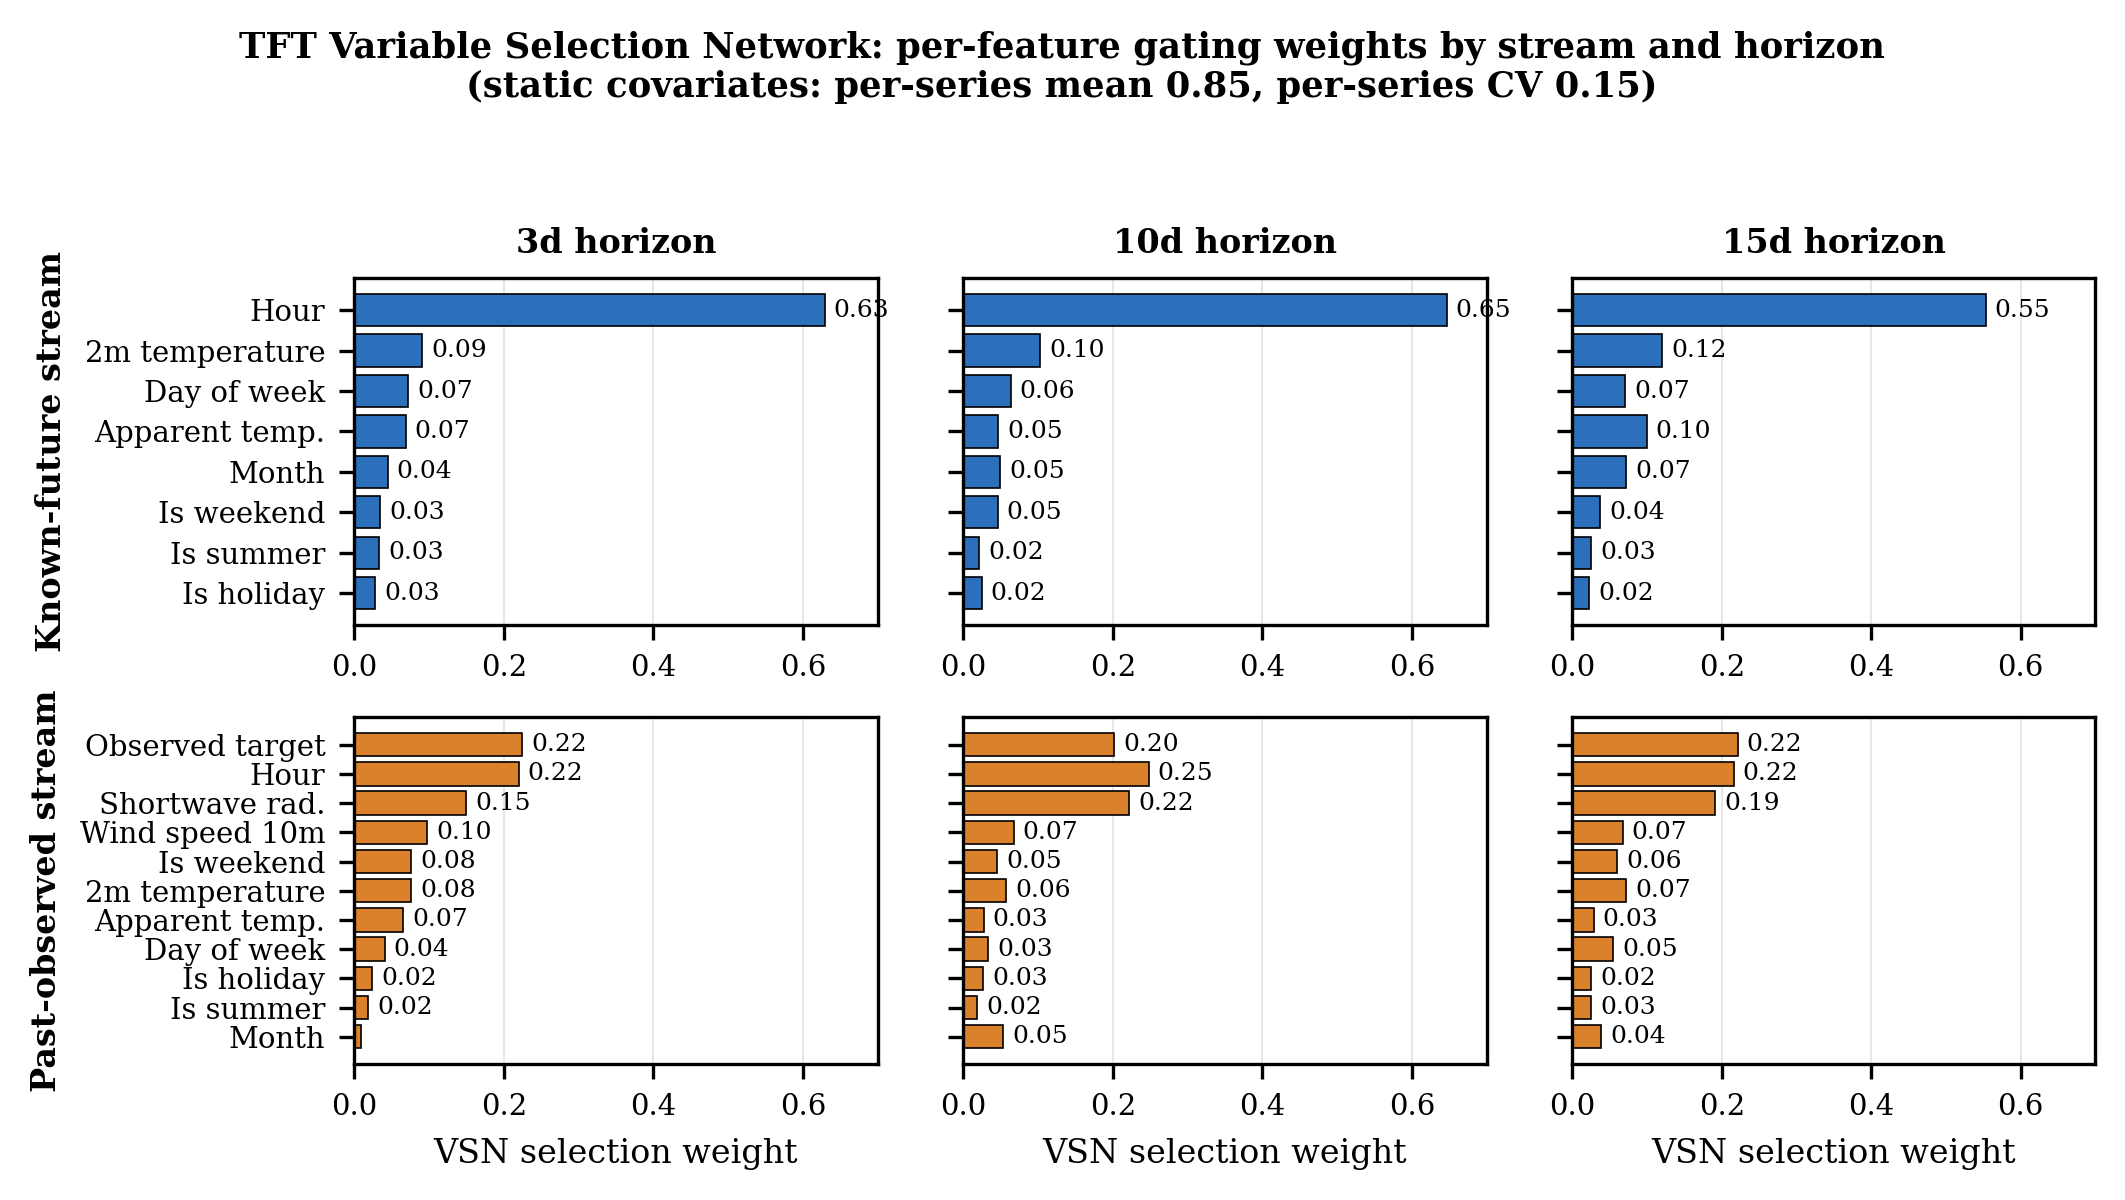
\includegraphics[width=\textwidth]{figures/fig_tft_vsn_importance.png}
    \end{center}
    \caption{TFT Variable Selection Network gating weights for the deployed 3-, 10- and 15-day models. Top row: known-future stream; bottom: past-observed. Weights sum to one within each stream; static covariates (not shown) are per-series mean 0.85, CV 0.15.}
    \label{fig:vsn}
\end{figure*}

\subsection{Feature and Hyperparameter Selection}

The TFT's feature set and hyperparameters are fixed in three phases, each scored on the walk-forward cross-validation of Section~\ref{sec:design}.

\subsubsection{Phase 1: Backward Feature Elimination}\label{sec:p1}

Phase 1 reduces the historical observed feature set from the seventeen available Open-Meteo variables to the smallest set that retains predictive accuracy, both to limit overfitting and to enable longer horizons within the GPU memory budget.

A backward-elimination loop drops, at each step, the least-important feature (lowest TFT variable-selection weight), re-evaluates all-year per-series relative MAE on walk-forward cross-validation, and keeps the lowest-error subset, with a loose early-stopping guardrail at twice the baseline error that never fired in practice, the error staying near-flat down to a single feature. The procedure was repeated for the variant that adds the scraped beach-attribute features as static inputs.

The backward-elimination process converges on a minimal set of two observed-weather features, shortwave radiation and vapour-pressure deficit, on an 11-beach development subset held out by a date cutoff. The best subset of that beach-attribute variant scores marginally lower but needs more features, so the scraped beach attributes are dropped from the deployed schema for parsimony rather than accuracy.

\subsubsection{Phase 2: Input-size Sweep}\label{sec:phase2}

The TFT's input window controls how much past history feeds the encoder. A shorter window may miss multi-day patterns; a longer window inflates training time and risks overfitting.

With features and hyperparameters held at the Phase-1 winner, the input size is swept over $\{12, 18, 24, 36, 48, 60, 72, 96, 120\}$ for each horizon, recording season relative MAE on walk-forward cross-validation with step and validation size both equal to the horizon.

Input size 48 minimises season relative MAE at every horizon; the error curve is U-shaped, so both shorter and longer windows do worse. The deployed models therefore use an input size of 48 daytime hours, the value the hyperparameter analysis of Section~\ref{sec:p3} also retains.

\subsubsection{Phase 3: Hyperparameter Search and Stability}\label{sec:p3}

This phase identifies the production hyperparameters and quantifies how stable
the optimum is to perturbations. The hypothesis emerged from a routine
observation\footnote{Recorded in the author's working notebook on 2026-03-12.}:
\emph{``dropout, hidden\_size, n\_head are constant --- the same value on HP
--- in different datasets''.} What follows is the formal validation of that
observation across 980+ trials, six search runs and a controlled
one-variable-at-a-time experiment.

The hyperparameter search history is highly iterative across consecutive development rounds. Optuna was used for the search phases (feature selection, input-size search), while the final hyperparameter step in the main training script uses a closed sweep of dropout over the range 0.0 to 0.3 (in steps of 0.02--0.05) with hidden size 64, four heads and a learning rate of $10^{-3}$. This configuration originates in the horizon-ceiling probe (see Section~\ref{sec:horizon_ceiling}) and was set on first-principles grounds before any empirical validation.

A controlled one-variable-at-a-time (OVAT) experiment measures the per-hyperparameter sensitivity at the FIXED-HP centre (Table~\ref{tab:ovat}). The dropout dimension is essentially flat across the interval $[0,\,0.3]$, justifying the production design of sweeping dropout while freezing the other three; the later P90-normalised cross-year search reproduces this flatness on $[0,0.3]$ in four of five completed cells, but finds it bounded: over a widened $[0,0.5]$ axis, dropout correlates positively with the loss on the curated dataset (Spearman $\rho$ up to $0.52$). The single sharp cliff is the learning rate above $5\!\times\!10^{-3}$ (Table~\ref{tab:ovat}).

A complementary, run-by-run check parses every best-of-run marker (the literal ``BEST'' or ``OPTIMAL HP'' lines) written across the full sequence of grid scripts and Optuna studies (100 distinct best-of-run entries in total) and tabulates which value of each hyperparameter was selected. The result is in Table~\ref{tab:bestcounts}. Hidden size 64 is the most frequently-selected value, learning rate near $10^{-3}$ wins more than half the runs, and FIXED-HP's exact triple appears as the run's overall best in 10 of 100 entries (or 17 if the learning rate is allowed to drift inside $[5\!\times\!10^{-4},\,1.5\!\times\!10^{-3}]$). The misses are uniformly distributed across neighbouring HP combinations rather than concentrated on a different optimum, consistent with the ``wide and flat optimisation surface'' interpretation in the OVAT analysis.

\begin{table}[!ht]
    \caption{FIXED-HP value frequency across 100 legacy best-of-run entries (\texttt{n\_head} was logged for 97 of them).}
    \label{tab:bestcounts}
    \begin{center}
    \footnotesize
    \begin{tabular}{lcc}
        \toprule
        Best-of-run hits FIXED-HP value of $\dots$ & count & share \\
        \midrule
        hidden\_size $= 64$           & 45 & 45\% \\
        \quad vs.\ $32$               & 23 & 23\% \\
        \quad vs.\ $128$              & 32 & 32\% \\
        n\_head $= 4$                 & 48 & 48\% \\
        \quad vs.\ $2$                & 47 & 47\% \\
        \quad vs.\ $8$                & 2  & 2\% \\
        $\eta = 10^{-3}$ exactly      & 29 & 29\% \\
        $\eta \in [5\!\times\!10^{-4},\,1.5\!\times\!10^{-3}]$ & 54 & 54\% \\
        \midrule
        \multicolumn{3}{l}{\emph{Joint matches}} \\
        $h{=}64 \land n_h{=}4 \land \eta = 10^{-3}$ exactly & 10 & 10\% \\
        $h{=}64 \land n_h{=}4 \land \eta \approx 10^{-3}$   & 17 & 17\% \\
        $h{=}64 \land n_h{=}4$ (any $\eta$)                 & 22 & 22\% \\
        $h{=}64 \land \eta \approx 10^{-3}$ (any $n_h$)     & 26 & 26\% \\
        \bottomrule
    \end{tabular}
    \end{center}
\end{table}

\begin{table}[!ht]
    \caption{One-variable-at-a-time sensitivity at FIXED-HP, 3-day horizon. Bold = FIXED-HP value. Dropout is flat; lr has a cliff at $5\!\times\!10^{-3}$.}
    \label{tab:ovat}
    \begin{center}
    \footnotesize
    \begin{tabular}{lcc}
        \toprule
        Hyperparameter & value & relMAE \\
        \midrule
        hidden size  & 32                   & 0.0464 \\
                     & \textbf{64}          & \textbf{0.0449} \\
                     & 128                  & 0.0498 \\
                     & 256                  & 0.0458 \\
        \midrule
        n.\ heads    & 2                    & 0.0452 \\
                     & \textbf{4}           & \textbf{0.0449} \\
                     & 8                    & 0.0472 \\
        \midrule
        dropout      & 0.0 to 0.3           & 0.0448 to 0.0450 \\
        \midrule
        learning rate & $5\!\times\!10^{-4}$ & 0.0459 \\
                      & $\boldsymbol{10^{-3}}$ & $\boldsymbol{0.0448}$ \\
                      & $2\!\times\!10^{-3}$ & 0.0473 \\
                      & $5\!\times\!10^{-3}$ & 0.0552 \\
        \bottomrule
    \end{tabular}
    \end{center}
\end{table}

The same conclusion held in a second, independent legacy sensitivity study where each parameter was perturbed across a wider range: learning rate and scaler type dominated that impact ranking, batch size and maximum number of steps were negligible, and hidden size and number of heads were intermediate, consistent with the OVAT result that perturbing them costs at most about 5\% relative MAE inside the search bounds. The cross-year re-examination (Table~\ref{tab:hp_perrun}) re-ranks these axes.

The per-run analysis aggregates more than 980 trials across six independent runs spanning the grid and Optuna phases. For each run, FIXED-HP-matching trials (trials whose hidden size, head count and learning rate equal the FIXED-HP values) are compared against the run's own best (Table~\ref{tab:hp_perrun}).

\begin{table}[!ht]
    \caption{FIXED-HP vs.\ per-run best: absolute relMAE deviation across 13 run-horizon cells.}
    \label{tab:hp_perrun}
    \begin{center}
    \footnotesize
    \begin{tabular}{lccc}
        \toprule
        Quantity & median & mean & max \\
        \midrule
        $\Delta$ rel.\ MAE  (FIXED vs.\ best) & $+0.0038$ & $+0.0041$ & $+0.0109$ \\
        $\Delta$ season    (FIXED vs.\ best)  & $+0.0022$ & $+0.0058$ & $+0.0222$ \\
        Within-run rel.\ MAE spread           & $0.029$   & ---       & $0.052$ \\
        \bottomrule
    \end{tabular}
    \end{center}
\end{table}

FIXED-HP is at most 0.011 absolute relative MAE worse than any run's individual best. The within-run spread (best vs.\ worst trial in a run) is five to thirteen times larger than this gap. FIXED-HP sits in the top 10--15\% of every run's hyperparameter space and is the operational choice; the roughly tenfold training-time saving from skipping hyperparameter search at every Phase-1 and Phase-2 trial substantially outweighs the at-most 1.1\% absolute loss.

An independent search run re-ran the search under the cross-year protocol (train on 2022 only, inner-validation within 2022, summer 2025 reserved as a frozen test window) with 200 TPE trials for each combination of model family and forecast horizon (a ``cell'') on two dataset variants, sharing one P90-normalised objective across TFT, LSTM and XGBoost. Three results refine the earlier findings. First, the per-cell optima relocate ($\eta \in [3.6\!\times\!10^{-5}, 5.3\!\times\!10^{-4}]$, $h \in [96, 256]$; the FIXED-HP triple was never sampled jointly in 899 completed TFT trials), yet the marginal penalty of each FIXED-HP value stays within $0.010$: the wide-flat interpretation survives, but its best point is dataset- and horizon-dependent rather than central. Second, the TFT fANOVA importance under that reduced grid is dominated by input size (top-three in all five completed TFT cells; window 48 wins every cell), dropout and hidden size follow on the second dataset variant, batch size is negligible in both search runs, and the 500-step trial budget favours smaller learning rates with longer early-stopping patience. Third, the budget is adequate: trials 100--200 improve the best-so-far trial by at most $0.0018$ absolute, and every 15-day trial with $h \geq 384$ fails on GPU memory, contracting the feasible space exactly where the model is largest. The frozen summer-2025 window is used for the TFT--LSTM significance test under the DM protocol of Section~\ref{sec:metric} (results in Section~\ref{sec:dm}).

The final consolidation search merged the Phase-1 and Phase-2 axes into one space and ran 150 TPE trials per family and horizon on the curated dataset, with a single per-series P90 objective so the fANOVA importances are comparable. For the TFT, three hyperparameters carry almost two thirds of the loss variance at the 15-day horizon (Figure~\ref{fig:hp_per_model}): the scaler (about 0.36), the learning rate (about 0.16) and the batch size (about 0.13). Every other axis (dropout, number of heads, hidden size, input size, attention dropout and early-stop patience) explains under 9 percent of the variance each. The other two families behave the same way: the scaler alone drives the LSTM (importance of about 0.71), and XGBoost is driven by its learning rate, column-sampling rate and tree depth. In every case a few axes decide the result and the rest can be fixed.

This is what the production pipeline does. It freezes three axes at sensible defaults (number of heads, batch size and early-stop patience) and searches the other six (scaler, learning rate, hidden size, input size, dropout and attention dropout) on each retrain. Fixing the rest cuts the per-trial training time, because the search no longer spends trials on axes that barely move the loss. The accuracy cost is small: a fixed-axis configuration stays close to the best run in Table~\ref{tab:hp_perrun}.

\begin{figure}[!t]
    \begin{center}
        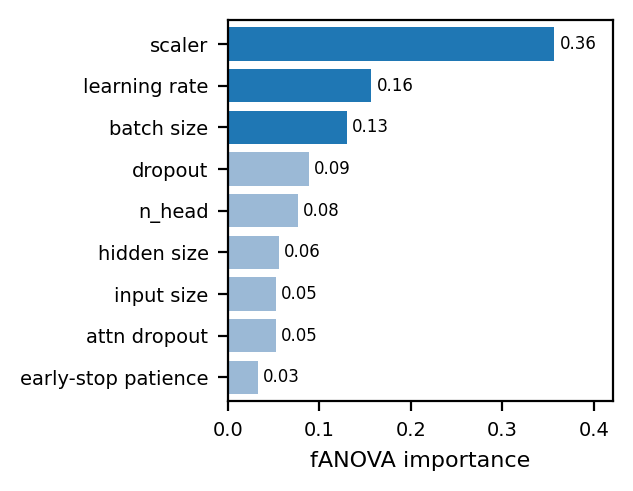
\includegraphics[width=0.92\columnwidth]{figures/fig_tft_fanova_importance.png}
    \end{center}
    \caption{TFT fANOVA hyperparameter importance at the 15-day horizon (unified 150-trial search, per-series P90 objective). The scaler (0.36), learning rate (0.16) and batch size (0.13) carry most of the loss variance (dark bars); the other axes each explain under 9\%.}
    \label{fig:hp_per_model}
\end{figure}

\section{Results and Analysis}\label{sec:results}

\subsection{Cross-year Daytime Result}\label{sec:xyear_result}

Evaluated on the daytime frame, Validation~1 separates the three families cleanly (Table~\ref{tab:daytime}). The TFT is the strongest at every horizon, with per-series P90 season relMAE $0.258$--$0.316$ against $0.310$--$0.424$ for the LSTM and $0.424$--$0.523$ for XGBoost: a $1.6$--$1.7\times$ margin over XGBoost and $1.2$--$1.3\times$ over the LSTM. The Diebold-Mariano test rejects equality of forecast accuracy in favour of the TFT against \emph{both} baselines at every horizon ($p<0.01$). XGBoost is the weakest here, probably because its recursive multi-step forecast accumulates error across the $195$ daytime hours, whereas the TFT emits the whole trajectory in a single pass. The hyperparameters are the per-family optima of the 150-trial unified search (see Section~\ref{sec:p3}), reused without re-searching: that search trains on the same 2022 era and the same daytime frame. It is tuned on a held-out 2022 inner-validation tail that never sees the test dataset, so it transfers directly to this protocol.

\begin{table}[!t]
    \caption{Cross-year daytime evaluation (Validation~1, train 2022, test the 2025--26 dataset; 13 beaches, matched rows). Per-series P90 season relMAE. The TFT wins every horizon, the Diebold-Mariano test is significantly better against both baselines ($p<0.01$).}
    \label{tab:daytime}
    \begin{center}
    \footnotesize
    \begin{tabular}{lccc}
        \toprule
        Horizon & TFT & LSTM & XGB \\
        \midrule
        3\,d  & \textbf{0.258} & 0.310 & 0.424 \\
        10\,d & \textbf{0.316} & 0.424 & 0.495 \\
        15\,d & \textbf{0.301} & 0.370 & 0.523 \\
        \bottomrule
    \end{tabular}
    \end{center}
\end{table}

\subsection{In-distribution Walk-forward}\label{sec:walkforward_result}

The walk-forward cross-validation of Validation~2 (see Section~\ref{sec:design}) re-runs the same cross-family comparison under the deployed system's operating condition, where recent in-distribution history is available. On the 13 beaches with enough history for the expanding folds, the TFT is again the strongest family: per-series P90 season relMAE of $14.6\%$ and $19.2\%$ at the 3- and 10-day horizons, against $22.1\%$ and $23.8\%$ for XGBoost and $26.3\%$ and $26.9\%$ for the LSTM. The Diebold-Mariano test confirms the advantage over both baselines at both horizons ($p<10^{-4}$ against XGBoost, $p<10^{-16}$ against the LSTM). Accuracy is clearly higher than the cross-year figures of Section~\ref{sec:xyear_result}, as expected when recent history is available, but the family ordering is unchanged.

\subsection{Baseline Comparison}\label{sec:baselines}

An early exploration compared the best-known regressors against a sequence-to-sequence LSTM on the preliminary 2022 data (15 beaches, daytime hours), to see how each family behaves before committing to an architecture (Table~\ref{tab:early_baselines}). Even with the tree and linear baselines tuned by Optuna, the LSTM led by a wide margin --- about half their mean absolute error and the only clearly positive $R^2$. The simpler regressors were therefore set aside; XGBoost alone was kept, because it is the method of the closest published study on this task: Castelle~\emph{et~al.}~\cite{Castelle2025} forecast hourly beach attendance from automatic video-derived counts and report a strong fit ($R^2{=}0.97$), making it the strongest literature-grounded tree-based reference to benchmark against (Section~\ref{sec:c2}). The final comparison then centres on three families carried through the full matched-rows protocol: that XGBoost reference, the recurrent LSTM, and the TFT.

\begin{table}[!ht]
    \caption{Early model-behaviour exploration on the preliminary 2022 data (15 beaches, daytime hours; tree and linear baselines Optuna-tuned). MAE in raw user counts. The sequence-to-sequence LSTM already dominates; XGBoost was kept as the published tree-based reference and the rest set aside.}
    \label{tab:early_baselines}
    \begin{center}
    \footnotesize
    \begin{tabular}{lcc}
        \toprule
        Model & Test MAE & Test $R^2$ \\
        \midrule
        LSTM (seq-to-seq)  & \textbf{17.4} & \textbf{0.55} \\
        Lasso              & 32.6 & 0.47 \\
        XGBoost            & 34.5 & 0.40 \\
        Gradient Boosting  & 39.7 & 0.20 \\
        Random Forest      & 51.8 & $-0.40$ \\
        \bottomrule
    \end{tabular}
    \end{center}
\end{table}

With the XGBoost reference fixed, the question is whether a sequence model, and then a deep attention model, justify their additional model capacity. To answer it fairly, the best LSTM, the best XGBoost and the best TFT were each tuned under one shared search budget and scored on the identical matched rows and the same per-series-P90 denominator (see Section~\ref{sec:design}). The ranking then reflects the architectures, not unequal tuning effort.

As established in Section~\ref{sec:metric}, the relevant metric is season relative MAE. On that metric the best LSTM is worse than the TFT at every horizon: the per-series P90 season relMAE of Table~\ref{tab:daytime} is $0.258$--$0.316$ for the TFT against $0.310$--$0.424$ for the LSTM, a gap that is Diebold-Mariano significant against both baselines. The tuned XGBoost captures day-of-week structure but underfits the weather-driven variation, and its cross-year transfer collapses to negative $R^2$ (see Section~\ref{sec:c2}). The residual error of every family concentrates in the high season (Jun--Aug), so the gap to the TFT is a genuine modelling gap rather than a seasonal or dataset artifact.

\subsection{Castelle-style XGBoost Replication}\label{sec:c2}

The model comparison starts from the published reference. Castelle~\emph{et al.}~\cite{Castelle2025} apply an XGBoost regressor on a single Atlantic beach (Biscarrosse) using air temperature (T), precipitation (P), wind speed (W), wind direction ($\alpha$) and insolation (I); humidity is not among their predictors. They report $R^2 = 0.97$ on hourly attendance. That accuracy does not transfer to the heterogeneous 22-beach Balearic dataset (Table~\ref{tab:c2}), so the XGBoost result on our data is the baseline reference for the recurrent and attention models. To test whether the same recipe transfers to the heterogeneous 22-beach Balearic dataset, a replication was implemented with two side-by-side configurations: \emph{curated} (the hand-cleaned 22-beach old-camera dataset) and \emph{cross-year} (train on 2022 rows only, test on summer 2025, the same stress test as scenario S1 for the TFT). Each configuration runs an Optuna~\cite{Akiba2019Optuna} 50-trial sweep over the standard XGBoost grid (number of estimators, maximum depth, learning rate, subsample, column-sample-by-tree and the two regularisation penalties) with autoregressive lag features and weather and calendar features computed from the unified dataset.

\begin{table}[!t]
    \caption{Castelle-style XGBoost on Jun--Aug 2025 (50 Optuna trials per cell). relMAE is P90-normalised; $R^2_\text{med}$ is the per-beach median.}
    \label{tab:c2}
    \begin{center}
    \footnotesize
    \setlength{\tabcolsep}{4pt}
    \begin{tabular}{lcccccc}
        \toprule
        & \multicolumn{2}{c}{3\,d} & \multicolumn{2}{c}{10\,d} & \multicolumn{2}{c}{15\,d} \\
        \cmidrule(r){2-3}\cmidrule(r){4-5}\cmidrule(r){6-7}
        Config & relMAE & $R^2_\text{med}$ & relMAE & $R^2_\text{med}$ & relMAE & $R^2_\text{med}$ \\
        \midrule
        curated    & \textbf{32.8\%} & \textbf{0.14} & \textbf{34.3\%} & \textbf{0.17} & \textbf{33.1\%} & \textbf{0.26} \\
        cross-year & 44.7\% & $-0.33$ & 41.0\% & $-0.09$ & 43.5\% & $-0.22$ \\
        \bottomrule
    \end{tabular}
    \end{center}
\end{table}

Table~\ref{tab:c2} yields two findings. First, XGBoost does not reach the TFT, but by a moderate margin: on the matched per-series-P90 metric of the main comparison (Table~\ref{tab:daytime}) the TFT leads both the recursive XGBoost and the LSTM by the margins reported there, all Diebold-Mariano significant. Second, and most informatively, cross-year transfer fails badly for XGBoost (41--45\% relMAE, \emph{negative} $R^2$: it stops tracking the variation at all) while the TFT degrades only gracefully (26--32\% relMAE, Section~\ref{sec:a2}, S1). The contrast isolates the architectural ingredient that matters: the TFT's autoregressive context (the previous hour's count and short rolling averages over recent daytime hours, fed as first-class inputs to its variable-selection network) and its gating mechanism over historical observed weather are what potentially allow it to transfer across years, while XGBoost's shifted-feature design has no comparable mechanism and does not transfer.

The $R^2$ gap to the published Castelle baseline (0.97 on a single Atlantic beach) is large: the 22-beach Balearic dataset gives a median $R^2$ of 0.26 at best (curated, 15-day) and negative $R^2$ on cross-year. Two factors drive the gap: the Balearic dataset spans 22 heterogeneous beaches with varying signal-to-noise, and webcam crowd counting on public cameras carries measurement noise --- low-light and occlusion failures, camera-specific artifacts and gaps --- that a controlled single-beach pipeline like Castelle's does not face. The XGBoost benchmark therefore confirms that the architectural step from XGBoost to TFT is necessary, not optional, on the heterogeneous Balearic dataset.

\subsection{Season-only Training: a Rejected Variant}

Tourist demand is concentrated in April through September. Training the model on summer-only data, or upweighting summer rows, might improve the operationally relevant high-season metric.

Three structurally distinct interventions were tried in sequence across consecutive development rounds: row-level duplication of summer months, a hard April--September filter with a max-capacity model, and a cutoff that trims the winter tail of training (specifically, cutting off training at 2025-10-30).

All three variants underperform uniform-sampling full-year training. The cutoff-vs-full comparison from the deployed pipeline is decisive (see Table~\ref{tab:cutoff_vs_full}). Full-year training wins at every horizon on the operational season metric. The row-duplication and the summer-filter both cleanly underperform. The combined evidence supports uniform-sampling full-year training as the final design.

\begin{table}[!ht]
    \caption{Season relMAE: cutoff-trained (one of the season-emphasis alternatives to full-year training) vs.\ full-year-trained TFT. Full-year wins at every horizon.}
    \label{tab:cutoff_vs_full}
    \begin{center}
    \begin{tabular}{lccc}
        \toprule
        Horizon & cutoff & full & $\Delta$ \\
        \midrule
         3\,d  & 0.2836 & \textbf{0.2257} & $+0.0579$ \\
        10\,d  & 0.2837 & \textbf{0.2553} & $+0.0284$ \\
        15\,d  & 0.2628 & \textbf{0.2379} & $+0.0249$ \\
        \bottomrule
    \end{tabular}
    \end{center}
\end{table}

\subsection{Dataset Comparison: the Curated Set Wins}

Three datasets were available at deployment time: a small 9-beach dataset (new cameras only), a 27-series dataset (new cameras plus old) and a 26-series curated dataset (old cameras, hand-cleaned: non-beach views and low-quality series removed manually). The same FIXED-HP model fitted on each and scored on a common test partition shows the 22-beach curated dataset winning at every horizon. The reason is image-quality regression: the new cameras were re-added through a server-side path that produced lower-quality snapshots, propagating into noisier counts and worse forecasts. Dataset choice is therefore driven by crowd-count-estimation quality, not by recency or dataset size, and the curated dataset is selected as the production training table. This manual quality filter is the step the automatic camera-validation screen (Figure~\ref{fig:camval}) is designed to replace, so that future dataset assembly, filtering and retraining run without hand-selection.

\subsection{Final Models and Deployed Numbers}

Three production models, one per horizon, are trained and frozen on the curated dataset, using the converged feature schema and hyperparameters.

The main training script\footnote{Final version dated 2026-03-12.} wraps the five sub-phases (horizon-limit probe, feature search, input-size search, hyperparameter grid, deploy) and offers a deploy-only fast path that skips the optimisation phases. Walk-forward cross-validation uses step and validation size both equal to the horizon, with five windows in production.

The deployed models' held-out accuracy is reported on a single, consistent metric throughout: the summer per-series P90 relMAE. The cross-year result is in Table~\ref{tab:daytime} and the production field evaluation on held-out post-deployment data in Table~\ref{tab:field_eval} (see Section~\ref{sec:prod}).

\subsection{Production Pipeline and Field Evaluation}\label{sec:prod}

The trained models move out of the offline notebook environment and into the BeachCamWeb Django application, where they serve forecasts on demand to both the operator dashboard and visitor-facing pages.

The production module under \texttt{apps/prediction} ships three pre-trained TFT model sets (3-day, 10-day, 15-day), a Django service that auto-selects a model by requested horizon (1--15~days), a feature-engineering pipeline that mirrors the offline schema (calendar features, weather backfill via Open-Meteo, holiday lookups via the Spanish holidays calendar), and a per-camera occupancy-classification layer that maps raw counts to four operational levels (\textsc{very-low}, \textsc{low}, \textsc{medium}, \textsc{high}) using per-beach max thresholds. A scheduled re-training job rebuilds the dataset and re-evaluates every candidate model against the most recent ten months of held-out data; the per-horizon best is promoted to production. The current dataset report and field-evaluation results are published at \url{https://ocupacioplatges.uib.eu/pipeline/report/}.

Validation~3 is the operational field evaluation: the production system periodically evaluates every candidate model set against the most recent ten months of held-out data and publishes the ranking on the operator dashboard. The production ranking is reported on the per-series P90 relMAE, the same denominator as the offline result (see Section~\ref{sec:metric}, Table~\ref{tab:daytime}), so the deployed models and the offline comparison are read on one scale.

The motivation for a continuously re-evaluated production ranking emerged
from a routine observation during the development phase. The author's
notebook records: \emph{``using the train dataset this approach is the best,
but when I ran on new dataset had a mix of results''.} The discrepancy
between cross-validation rankings on the training dataset and rankings on
held-out post-deployment data is therefore not an artifact to be
explained away but a known feature of the deployment setting that motivates
the re-evaluation cadence built into the production pipeline.

The ranking as of the most recent re-train (Table~\ref{tab:field_eval}) shows the TFT winning at every horizon on the deployed 13-bucket frame: summer per-series P90 relMAE of 19--26\%, ahead of the LSTM by 41--72\% relative and XGBoost by 80--97\%. This matches the offline ranking of Section~\ref{sec:baselines} on held-out post-deployment data.

Beyond the periodic ranking, the operator dashboard exposes a side-by-side hindcast comparison that any user can drive. They pick a past date, a forecast length, and up to three candidate model sets; the system replays the forecast each model would have produced for that window and overlays the realised occupancy on the same hourly grid. The candidate sets are trained on different data and protocols (the deployed TFT, the LSTM and XGBoost baselines, and the cross-year, full-season and recent-month variants of Section~\ref{sec:a2}), so the user sees directly how the choice of training data and model family plays out on a window they choose. The view reports, per model, the cross-validation relMAE, the summer- and season-subset relMAEs, and a hindcast relMAE specific to the selected window; clicking any bar loads the original webcam snapshot and the per-camera density map for that hour, and a per-hour tooltip lists every input feature the model received. Because the comparison runs live, any user can reproduce the published ranking on a window of their choice rather than take it on trust. It complements the multi-scenario evaluation of Section~\ref{sec:a2}: Table~\ref{tab:a2} reports the aggregate result, while this view lets a reader inspect it case by case.

\begin{table}[!ht]
    \caption{Production field evaluation over the full deployment range (Apr 2025--Jun 2026): summer (Jun--Aug) per-series P90 relMAE (mean $\pm$ SD across walk-forward windows; $n=999/397/267$ at 3/10/15\,d). ``vs.\ best'' is the penalty against the TFT.}
    \label{tab:field_eval}
    \begin{center}
    \footnotesize
    \begin{tabular}{llcc}
        \toprule
        Horizon & Model & summer relMAE (P90, \%) $\pm$ SD & vs.\ best \\
        \midrule
         3\,d & $\star$ TFT  & \textbf{18.8} $\pm$ 9.4 & --- \\
              & LSTM         & 32.3 $\pm$ 14.3 & $+72\%$ \\
              & XGB          & 33.9 $\pm$ 40.0 & $+80\%$ \\
        \midrule
        10\,d & $\star$ TFT  & \textbf{23.1} $\pm$ 11.8 & --- \\
              & LSTM         & 33.0 $\pm$ 12.6 & $+43\%$ \\
              & XGB          & 45.4 $\pm$ 44.7 & $+97\%$ \\
        \midrule
        15\,d & $\star$ TFT  & \textbf{26.0} $\pm$ 14.9 & --- \\
              & LSTM         & 36.6 $\pm$ 14.0 & $+41\%$ \\
              & XGB          & 47.4 $\pm$ 39.8 & $+82\%$ \\
        \bottomrule
    \end{tabular}
    \end{center}
\end{table}

\subsection{Multi-scenario Independent Validation}\label{sec:a2}

The cross-year comparison (Table~\ref{tab:daytime}) rests on a single split. Validation~4 confirms the ranking is not specific to that one window by re-scoring the same three families (TFT, LSTM and recursive XGBoost) on three independent daytime windows. The windows form a difficulty gradient, set by how far the test period sits from the training data. \emph{S1} (cross-year) is the hardest: it trains on 2022 alone and tests on Jun--Aug 2025, three years later. \emph{S2} (full-season) trains through March 2025 and tests on Apr--Sep 2025, so training and test share the same era. \emph{S3} (recent-month) is the easiest: it trains through August and tests on September 2025, where the two periods almost meet. Within every window each family issues the same 195-hour daytime trajectory from the same weekly origins and is scored on the same per-series-P90 denominator, so each cell is a paired, like-for-like comparison. Each window keeps only the beaches with enough history before its training cut-off to condition the static covariates: 13 for S1, 12--13 for S3, but only 4 for S2. S2 is the narrowest check because its full-season split needs data before April 2025, which only the four beaches spanning both the 2022 and 2025 eras have.

\begin{table*}[!t]
    \caption{Fair multi-scenario daytime validation (8:00--20:00 frame, same 195-hour 15-day trajectory): per-series P90 relMAE (\%), paired per-row; bold = best per column. Beaches per window: S1~13, S2~4, S3~12--13.}
    \label{tab:a2}
    \begin{center}
    \footnotesize
    \begin{tabular}{l ccc ccc ccc}
        \toprule
        & \multicolumn{3}{c}{S1: cross-year} & \multicolumn{3}{c}{S2: full season} & \multicolumn{3}{c}{S3: recent month} \\
        \cmidrule(lr){2-4}\cmidrule(lr){5-7}\cmidrule(lr){8-10}
        Model & 3\,d & 10\,d & 15\,d & 3\,d & 10\,d & 15\,d & 3\,d & 10\,d & 15\,d \\
        \midrule
        TFT  & \textbf{26.1} & \textbf{32.4} & \textbf{30.5} & \textbf{24.6} & \textbf{30.1} & \textbf{27.1} & \textbf{16.4} & \textbf{19.9} & \textbf{18.2} \\
        LSTM & 31.3 & 42.5 & 38.8 & 25.7 & 37.2 & 29.9 & 17.0 & 30.6 & 18.9 \\
        XGB  & 43.0 & 50.8 & 53.0 & 35.0 & 38.8 & 39.4 & 21.6 & 26.7 & 28.0 \\
        \bottomrule
    \end{tabular}
    \end{center}
\end{table*}

Three findings stand out (Table~\ref{tab:a2}). First, the TFT wins every scenario at every horizon, Diebold-Mariano significant against both baselines in all eighteen comparisons. The ranking TFT $>$ LSTM $>$ XGBoost is therefore stable across these three independent windows, not an artifact of the main split. Second, the cross-year S1 column closely tracks the result of Table~\ref{tab:daytime} (TFT 26.1 / 32.4 / 30.5\% on the S1 summer window against the season figures 25.8 / 31.6 / 30.1\% there), confirming the cache2022 result is not specific to its evaluation window. Third, all three families ease from S1 (cross-year, the hardest case, eras three years apart) through S2 to S3 (recent-month, where the eras nearly meet), and XGBoost stays the weakest family throughout (43--53\% on S1, 35--39\% on S2, 22--28\% on S3): its recursive one-step iteration accumulates error over the 195-hour daytime trajectory, and its cross-year degradation is the largest of the three, consistent with the negative $R^2$ reported in Section~\ref{sec:c2}. The S2 column rests on only four beaches (those with pre-April-2025 history), so it is the least robust of the three windows.

This check uses the same per-series-P90 denominator as the main result, so its numbers are directly comparable to Table~\ref{tab:daytime}. It answers a different question from the deployed-model ranking of Section~\ref{sec:prod} (Table~\ref{tab:field_eval}), which scores the production \emph{checkpoints} to decide which snapshot to serve.

\subsection{Statistical Significance (Diebold-Mariano)}\label{sec:dm}

Two design claims are tested for significance under the Diebold-Mariano (DM) protocol of Section~\ref{sec:metric}: whether the three dedicated horizon models are justified over a single 15-day model, and whether the step from the baselines (LSTM and XGBoost) to the TFT is real rather than an artifact of a particular evaluation window. The first test re-runs the deployed models through the BeachCamWeb prediction service on the frozen summer-2025 window (1~June--31~August); the second uses the matched 15-day daytime evaluation of Table~\ref{tab:daytime}, where every family issues the same 195-hour daytime trajectory. Both pair every competing forecast observation-for-observation on \emph{identical} targets: the same cameras, the same daytime hours (8:00--20:00), and the same forecast origins. The loss is the absolute error in raw user-count units (consistent with the MAE metric and invariant to the per-series normalisation), and the Newey--West HAC variance~\cite{NeweyWest1987} is computed within each beach-window block. A negative DM statistic favours the first-named model.

Are three horizon models necessary? To test whether a dedicated short-horizon model earns its place, the production TFT is issued at all three horizons from a common grid of forecast origins, and the dedicated 3- and 10-day forecasts are compared against the 15-day model \emph{truncated} to the same lead window on identical targets (Table~\ref{tab:dmh}). The dedicated 3-day model is substantially better than truncating the 15-day model: summer MAE $13.6$ vs $16.4$ users (a $17\%$ reduction), DM $=-7.8$, $p\approx5\times10^{-15}$ (Wilcoxon $p\approx10^{-153}$). The dedicated 10-day model, in contrast, does \emph{not} significantly beat the truncated 15-day model: summer MAE $17.4$ vs $17.6$ (a $1\%$ edge), DM $=-0.7$, $p=0.46$ (Wilcoxon $p=0.08$). The DM therefore justifies the dedicated short-horizon model clearly but not the 10-day one: the dedicated 3-day model contributes a large, significant gain at the horizon where operational precision matters most, whereas the 10-day model adds only a small, statistically insignificant edge over reading the first ten days off the 15-day model. A single 15-day model would give up meaningful 3-day accuracy; the 10-day model is retained for operational symmetry across the three published horizons rather than for a demonstrated accuracy gain.

\begin{table}[!t]
    \caption{DM test: dedicated TFT model vs.\ the 15-day model truncated to the same horizon, summer 2025, paired per-row. MAE in users; negative DM favours the dedicated model.}
    \label{tab:dmh}
    \begin{center}
    \footnotesize
    \setlength{\tabcolsep}{4pt}
    \begin{tabular}{lccccc}
        \toprule
        Comparison & $n$ pairs & MAE$_\text{ded}$ & MAE$_{15\text{d}}$ & DM & $p_\text{DM}$ \\
        \midrule
        3\,d\ vs\ 15\,d$[:3]$   & 13{,}860 & \textbf{13.6} & 16.4 & $-7.8$ & $5\!\times\!10^{-15}$ \\
        10\,d\ vs\ 15\,d$[:10]$ & 46{,}048 & 17.4 & 17.6 & $-0.7$ & $0.46$ \\
        \bottomrule
    \end{tabular}
    \end{center}
\end{table}

Are the TFT's gains over the baselines significant? On the matched 15-day daytime evaluation (where all three families issue the same 195-hour daytime trajectory from the same weekly origins, so every forecast is paired observation-for-observation, Table~\ref{tab:daytime}), the Diebold-Mariano test confirms the TFT's advantage against \emph{both} baselines at every horizon (Table~\ref{tab:dm}). The TFT carries the lower per-row loss with DM statistics from $-16$ to $-47$ (negative favours the TFT) and $p$ from $10^{-53}$ down to numerical underflow, reproduced by the Wilcoxon signed-rank check ($p\approx0$); the MAE reduction is $26$--$28\%$ over the LSTM and $42$--$50\%$ over XGBoost. This fair pairing is what the deployed comparison of Section~\ref{sec:prod} could not provide: the deployed XGBoost used a 24-hour sliding-window scheme that did not share the forecast origins (so it is not origin-matched for a paired DM test there), and the deployed LSTM was under-tuned, inflating its \emph{operational} gap to roughly $2\times$; the equal-budget statistical comparison here narrows the TFT--LSTM margin to $1.2$--$1.3\times$ (and the TFT--XGBoost margin to $1.6$--$1.7\times$) while keeping both decisively significant.

\begin{table}[!t]
    \caption{Diebold-Mariano test, TFT vs.\ each baseline on the matched 15-day daytime evaluation (cache2022, 13 beaches, paired per-row). MAE in raw user counts; negative DM favours the TFT. Wilcoxon $p\approx0$ throughout.}
    \label{tab:dm}
    \begin{center}
    \footnotesize
    \begin{tabular}{llcccc}
        \toprule
        Horizon & vs.\ & MAE$_\text{TFT}$ & MAE$_\text{base}$ & DM & $p_\text{DM}$ \\
        \midrule
         3\,d  & LSTM & \textbf{13.8} & 18.7 & $-15.6$ & $<10^{-53}$  \\
               & XGB  & \textbf{13.8} & 25.6 & $-25.6$ & $<10^{-140}$ \\
        \midrule
        10\,d  & LSTM & \textbf{17.4} & 24.1 & $-33.3$ & $<10^{-240}$ \\
               & XGB  & \textbf{17.4} & 30.0 & $-35.2$ & $<10^{-267}$ \\
        \midrule
        15\,d  & LSTM & \textbf{16.3} & 22.0 & $-23.0$ & $<10^{-116}$ \\
               & XGB  & \textbf{16.3} & 32.5 & $-46.7$ & ${\approx}\,0$ \\
        \bottomrule
    \end{tabular}
    \end{center}
\end{table}

\subsection{Per-horizon Feature Schema in Production}\label{sec:prodfeat}

A second item published alongside the ranking for transparency is the input feature schema of the deployed model (Table~\ref{tab:prod_features}). The production winner uses a single fixed schema across all three horizons, the converged output of the feature-elimination analysis in Section~\ref{sec:tftfeat}: a known-future weather triplet (temperature, apparent temperature, cloud cover) grounded on forecast-stability theory and tourism-climate-index canon, three observed-only weather signals (low cloud cover, shortwave radiation, vapour-pressure deficit), the five calendar features (hour, day-of-week, month, is\_weekend, is\_summer), and two per-series static covariates (the beach mean and its coefficient of variation). Fixing one small schema across the three horizons keeps the production pipeline simple and the per-feature attributions directly comparable across the deployed models.

\begin{table}[!ht]
    \caption{Feature schema of the production winner, identical across the 3-, 10- and 15-day horizons. FUTURE: known at forecast time. OBSERVED-ONLY: observed only.}
    \label{tab:prod_features}
    \begin{center}
    \footnotesize
    \begin{tabular}{ll}
        \toprule
        Type & Features \\
        \midrule
        FUTURE weather  & 2m temperature, apparent temperature, \\
              & \quad cloud cover \\
        FUTURE calendar & hour, day-of-week, month, \\
              & \quad is\_weekend, is\_summer \\
        OBSERVED-ONLY weather  & low cloud cover, shortwave radiation, \\
                      & \quad vapour-pressure deficit \\
        Static        & per-series mean, coefficient of variation \\
        \midrule
        \multicolumn{2}{l}{Total: 8 future-known + 3 observed + 2 static} \\
        \bottomrule
    \end{tabular}
    \end{center}
\end{table}

The deployed schema matches the minimal set that backward elimination converged on in Section~\ref{sec:p1}: the production winner keeps the small observed-weather set (shortwave radiation and vapour-pressure deficit, plus low cloud cover) rather than a richer per-horizon one, confirming the feature-elimination finding transfers to the full production dataset.

\subsection{Day-type and Calendar Effects}\label{sec:daytype}

Beach occupancy follows a calendar structure (weekday vs.\ weekend, ordinary day vs.\ holiday) that interacts with the seasonal cycle. This subsection quantifies the size of these effects on the production dataset and confirms the calendar features (is\_weekend, is\_holiday-derived features, day\_of\_week) carry signal beyond the trivial weekday/weekend split.

The dataset report aggregates each row by day type and month for all 22 beaches; Figure~\ref{fig:monthly_daytype} shows the mean crowd per month by day type and the holiday count per month.

Two findings stand out (Figure~\ref{fig:monthly_daytype}). First, the weekend uplift is largest in shoulder months (May, September) where weekday demand is low and weekenders dominate; in peak summer the weekday and weekend means nearly coincide because daily tourist demand fills the beaches regardless of the day of the week. Second, holidays produce a heterogeneous per-beach signal: individual beaches show $+30\%$ to $+40\%$ holiday uplift on summer holidays, but others show negative uplift (probably weekday-commuter or working-locals beaches that empty on holidays). This heterogeneity supports the argument in the Future Work section for per-beach hierarchical training: a global is\_holiday feature averages out a signal that is genuinely beach-specific.

\begin{figure*}[!t]
    \begin{center}
        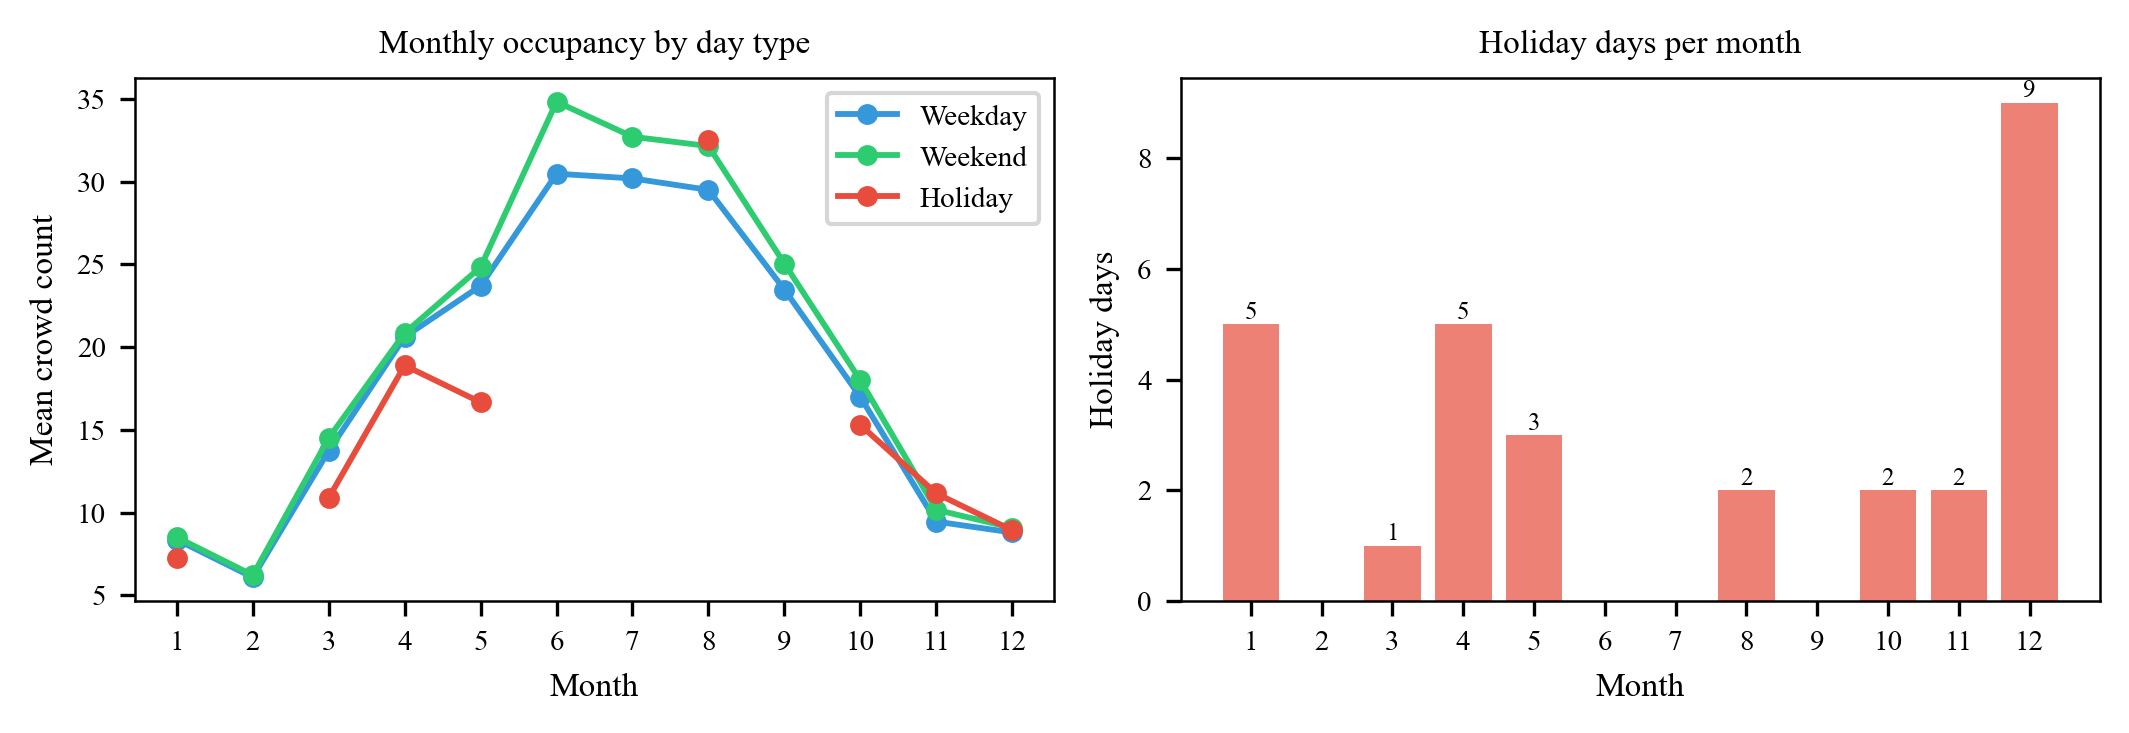
\includegraphics[width=\linewidth]{figures/fig_monthly_by_daytype.png}
    \end{center}
    \caption{Mean crowd per month by day type (left) and number of holidays per month (right).}
    \label{fig:monthly_daytype}
\end{figure*}

\subsection{Horizon Ceiling Probe}\label{sec:horizon_ceiling}

A standalone probe quantifies the maximum forecast horizon the TFT can be trained on under the deployment hardware (RTX A6000, 48~GB). This is a training-limit test, not a production setting: the deployed system forecasts only 3, 10 and 15 days, and the longer horizons below are never served. The probe runs a coarse-to-fine search over $H \in \{168, 360, 444, 528, 720, 1080, 1440, 2160\}$ hours with FIXED-HP and input size 48, training the same architecture from scratch on the 26-series dataset at each horizon and recording season relative MAE.

The ceiling is $H{=}444$ output steps (34 days on the thirteen-hour frame), with season relative MAE 0.189. Adjacent points: $H{=}360$ (28 days) trains cleanly at season relMAE 0.136 and $H{=}168$ (13 days) at 0.155; $H{=}528$ (41 days), $H{=}720$, $H{=}1080$, $H{=}1440$ and $H{=}2160$ all fail with out-of-memory before training completes. Performance is non-monotonic in horizon: the $H{=}360$ point is the best on season relMAE (0.136), ahead of the $H{=}168$ and $H{=}444$ points, so accuracy improves from $H{=}168$ to $H{=}360$ and then degrades by roughly 0.05 absolute at $H{=}444$, consistent with the TFT having marginally more difficulty as the future-known weather context weakens. A separate hyperparameter sweep at $H{=}444$ reconfirms FIXED-HP as the optimum on that horizon ($h{=}64, n_h{=}4, \text{dropout}{=}0.05, \eta{=}10^{-3}$, input 48), strengthening the stability claim of Section~\ref{sec:p3} on the limit-horizon setting where the model is most sensitive.

The $H{=}444$-step ceiling (34 days on the thirteen-hour frame) exceeds the 16-day Open-Meteo API cap by roughly $2.1\times$, so the operational bottleneck is forecast availability, not model capacity. Migration to the Open-Meteo seasonal-forecast API (35-day GFS coverage) would be supported by the existing hardware without retraining the architecture.

\section{Discussion}

\subsection{What Worked}

The convergence of three independent lines of evidence on the same FUTURE weather triplet (predictability theory, tourism-climate-index canon and direct precedent in Castelle~\emph{et al.}~\cite{Castelle2025}) supports the choice, though generalisation beyond the Balearic setting is untested. The empirical FIXED-HP stability finding (a wide, flat optimisation surface whose best point drifts with dataset and horizon but whose plateau penalty stays below 0.01 relative MAE, Section~\ref{sec:p3}) means future deployments can re-train without re-tuning at a small, quantified cost, simplifying production maintenance.

\subsection{What Did Not Work}

Season-only training, in all three variants, underperformed uniform full-year training: the intuition that ``the model should specialise on the regime that matters'' was not borne out.

\subsection{Limitations}

\textit{Ground-truth quality.} Forecast accuracy is bounded by the Bayesian VGG-19 crowd counting model's accuracy on Balearic webcams. Every error figure in this thesis is measured against the crowd counting model's estimated counts, which are the modelling target, not against true human occupancy: the dataset itself is generated by the crowd counting model, so there is no independent ground truth for the forecast. The crowd counting model's own deviation from a real human count is a separate, upstream error that these forecast metrics do not capture. Manual annotations were produced to fine-tune the crowd counting model, but the labelled set is small relative to the scale required to push the crowd counting model past its current calibration ceiling, and no per-beach human-labelled validation set is reserved for this thesis. The camera-validation filter (seasonality slope, Cohen's $d$) removes obviously broken cameras but cannot quantify the crowd counting model's residual error on the surviving series. These are public webcams operated by third parties and used through whatever access was available, not cameras deployed or selected for this study, so their placement, framing and uptime lie outside the project's control. Three concrete camera-side noise sources follow directly: cameras that physically pan, tilt or zoom across the day, introducing field-of-view drift that the crowd counting model sees as crowd-count shifts; cameras that turn off intermittently, leaving gaps the daytime filter does not fully reconstruct; and heterogeneous image quality across providers (resolution, compression artifacts, lens distortion), which directly affects the density-map regression.

These data-quality bounds are real, but the pipeline reduces them over time: the production system in Section~\ref{sec:prod} writes every snapshot, every predicted count, and every realised occupancy back to the dataset store. As the deployment accumulates additional months of cleaner imagery from the better-behaved cameras (and as flagged or moving cameras are pruned or replaced), each scheduled re-train ingests a progressively higher-quality training distribution. As more clean data accumulates across retraining cycles, the training distribution improves, so accuracy on later panels may improve as well; whether it does is an empirical question for future data.

\textit{Spatial coverage.} Each estimate reflects only what a camera's field of view captures. On a large beach a single (or a handful of) fixed camera(s) cannot frame the whole sand: the system measures occupancy on the covered area and treats it as a proxy for the beach as a whole, while stretches without a camera are never observed. The reported occupancy is therefore conditional on the existing camera placement and can under- or over-represent the true beach-wide crowd wherever coverage is partial; estimating whole-beach occupancy directly would require denser or wider-angle camera deployment.

\textit{Dataset coverage and temporal gaps.} The dataset is built from two disjoint collection eras (a 2022 cache and the 2025--2026 deployment) separated by a multi-year gap with only sparse 2023 data in between. Across that gap the underlying process drifts: tourism volume and seasonality, beach popularity, and the cameras themselves (replacement, relocation, re-framing) all change, so a model trained on one era need not transfer to the other: the cross-year stress test (see Section~\ref{sec:design}) shows a beach busy in 2022 but quiet in 2025 being systematically over-predicted. Within each era the series are gappy too: cameras drop offline, the collection pipeline halts on server faults, image resolution and provider change over time, and a camera's field of view shifts when it is panned, tilted, zoomed or physically moved. These interruptions break the hourly continuity the models assume and inject non-stationarity that is neither weather- nor calendar-driven; the reindex-and-pad step restores a continuous grid for training but cannot recover the missing observations. Future work follows directly: a continuously monitored collection pipeline with fail-over and alerting to avoid multi-day outages, explicit camera-stability checks (field-of-view and exposure-drift detection) so re-framed cameras are flagged rather than silently mixed into a series, and longer uninterrupted coverage that bridges the era gap, so cross-year training is no longer a transfer across distinct eras.

\textit{Two-era dataset.} The 2022 cache and 2025 Django data have different camera hardware, different framing and different image-quality conditions. The unified dataset relies on the haversine matching to bridge them, but a per-camera calibration was not performed. The two eras are also stored on different clocks: the 2025--2026 Django rows are in UTC and the 2022 cache in Madrid local time, so the fixed 8:00--20:00 window sits about one to two hours later in local time for the 2025--2026 rows. The weather features are aligned to the true instants, so the inputs are not corrupted, but the calendar hour-of-day feature carries this offset between eras.

\textit{Forecast input chain.} At inference time the FUTURE weather inputs are themselves forecasts from Open-Meteo, with their own decay in skill past day 7--10~\cite{ECMWF2024}. The deployed numbers in this thesis use the ground-truth (post-hoc) weather; the operational error includes the forecast cascade and is expected to be moderately worse, particularly at the 15-day horizon.

\textit{Uncertainty quantification.} Predictive intervals are produced by the framework's quantile heads but were not benchmarked against a calibration target. Operational deployment would benefit from explicit conformal-prediction wrappers.



\subsection{Reproducibility}\label{sec:repro}

\textit{Code and data.} All code is in the \texttt{beachcamweb} repository\footnote{\url{https://github.com/antoni-oliver/beachcamweb}}, on \texttt{main} at commit \texttt{a4c8996}, the deployed state of the running system at \url{https://ocupacioplatges.uib.eu/}.
The dataset is assembled by \texttt{build\_dataset\_v4.py} (the Django/cache merge with weather enrichment), cleaned by \texttt{generate\_train\_data.ipynb} (the 8:00--20:00 daytime filter, stuck-camera and seasonality removal, and a $\geq$1000-row cardinality filter) and exported in raw form; the per-series P90 outlier cap ($k=1.5$, applied to the ground-truth target only, never to predictions) is then applied at load time.

\textit{Provenance.} Each training run records its full invariants (dataset, train/test windows, metric definition, daytime window, season and summer-month sets, capacity definition, hyperparameter search space and library versions) in a \texttt{protocol.json}, and every hyperparameter trial persists to an Optuna SQLite study; the seed and software environment are in Section~\ref{sec:setup}.

\section{Conclusions and Future Work}\label{sec:conclusion}

This thesis presents a multi-horizon forecasting pipeline for hourly daytime beach occupancy on 26 series in the Balearic Islands, deployed at horizons of 3, 10 and 15 days inside the BeachCamWeb production system. The Temporal Fusion Transformer is the strongest model at every horizon: on the matched per-series-P90 statistical metric (Table~\ref{tab:daytime}) it beats a tuned recursive XGBoost by $1.6$--$1.7\times$ and an equally-tuned LSTM by $1.2$--$1.3\times$, Diebold-Mariano significant against both ($p<0.01$). Continuously re-evaluated against held-out 2025--2026 data, the production winner reaches summer per-series P90 relMAE of 18.8\%, 23.1\% and 26.0\% across the three horizons, against 32.3\%, 33.0\% and 36.6\% for the deployed LSTM (Table~\ref{tab:field_eval}); this deployed gap is wider than the equal-budget statistical comparison above, partly because the deployed LSTM uses fixed rather than fully searched hyperparameters. The work contributes a unified hourly dataset from heterogeneous 2022 and 2025 sources, a documented sequence of design experiments including feature elimination, hyperparameter stability and dataset comparison, negative results on season-only training and AEMET integration that informed the final design, and a transparency layer that publishes the cross-validation ranking and the feature schema for every candidate model. Throughout, the summer and season metrics are emphasised over the all-year metric for the reasons established in Section~\ref{sec:metric}.

Several directions follow. Three concern the model. First, per-beach hierarchical training to handle the heterogeneity in signal-to-noise across small and large, remote and urban beaches. Second, explicit holiday-week peak modelling to attack the largest residuals in June through August. Third, conformal-prediction~\cite{Angelopoulos2023Conformal} wrappers for calibrated predictive intervals at the operationally relevant 7-day horizon. Two more concern the data. The dataset still has gaps and a multi-year break between the 2022 and 2025 collection eras, and several beaches lack complete summer and season coverage; a continuously monitored collection pipeline, with fail-over and longer uninterrupted records, would give denser and more balanced summer and season data and remove the cross-era transfer problem. Finally, the counts depend on a Bayesian VGG-19 crowd counting model applied to public webcams, so higher-resolution imagery and a crowd counting model validated against hand-labelled Balearic frames would give more accurate people estimates and raise the ceiling on every downstream forecast.



\section*{Declaration on the Use of AI Tools}

Generative artificial-intelligence assistants were used during the preparation of this thesis strictly as productivity tools, under the author's direction and subject to the author's verification. Two assistants were used. Anthropic Claude assisted with the analysis, evaluation and training code and the \LaTeX{} scaffolding (from the author's specifications), with refining the English prose for clarity and academic register, with maintaining a running methodological log of the design decisions, and as a sounding board for methodological choices such as the statistical-significance tests. Google NotebookLM was used for grounded summarisation of, and question-answering over, the source literature and the author's own working notes, to navigate and cross-check references. Every figure, table, numeric result, modelling decision, experimental outcome and bibliographic reference was verified or reproduced by the author against the underlying data and code; no AI assistant generated experimental results, made design decisions, or selected references without subsequent human verification. The author retains full responsibility for the content and for any errors that remain.



\bibliographystyle{abbrv}
\bibliography{bibliography}

\end{document}
